% pic01.jpg = 20261011_121022832.jpg; Drive ID: 1mA9Cnh-2NLh2j1PvI0zL_4Dvw6U0OLCd
% pic02.jpg = 20261011_121038628.jpg; Drive ID: 1HhJhn7qh8zbR5ZuSaebOEAki1mOfQJmb
% pic03.jpg = 20261011_121046667.jpg; Drive ID: 1QHn55vxyi9G73eTxGFLkkFsNzUwAgXmq
% pic04.jpg = 20261011_121058449.jpg; Drive ID: 1t4GyMjNTFMcyFbl2Fb8UrRiEeexYkyjw
% pic05.jpg = 20261011_121102894.jpg; Drive ID: 13wtoeao5o1nt7PuGMWlErPks4oX49ecM
% pic06.jpg = 20261011_121115043.jpg; Drive ID: 1xn9zlBRTq8OnJ3mfvboy_ucH-Pos9S8G
% pic07.jpg = 20261011_121119559.jpg; Drive ID: 1ZS0f6ho0694ocwRe7MMF5cjwcscVz1LS
% pic08.jpg = 20261011_121133751.jpg; Drive ID: 1feBa4u7HNI3JeHr-2FMbBydNhwn25pdt
% pic09.jpg = 20261011_121142023.jpg; Drive ID: 1eq8dW3oOxFj6VYfdtg6EgrbSiXSCCeCr
% pic10.jpg = 20261011_121159146.jpg; Drive ID: 1CJUxTh3qEIvmb0FPJOADeRNMSm6rU2_M
% pic11.jpg = 20261011_121205075.jpg; Drive ID: 1_qvTgr3bFpAWZNC4Wc2BBc-eJsViUMMN
% pic12.jpg = 20261011_121216949.jpg; Drive ID: 14coIbJn3hBSb-a3MegM-IJm538e5a1nM
% !TeX program = xelatex
% UTF-8. Compile from this directory: xelatex STI.tex
% Define \STIInNotebook before inputting this file into an existing XePersian document.
% Source: Google Drive Notebook/STI; images ordered by original filename.
\ifdefined\STIInNotebook
  \let\STIfinish\relax
\else
  \def\STIfinish{\end{document}}
  \documentclass[12pt,a4paper]{article}
  \usepackage[margin=22mm]{geometry}
  \usepackage{amsmath,amssymb}
  \usepackage{graphicx}
  \usepackage{array,longtable}
  \usepackage{xepersian}
  \IfFontExistsTF{Amiri}{\settextfont{Amiri}}{\settextfont{DejaVu Sans}}
  \setlatintextfont{DejaVu Serif}
  \setlength{\parindent}{0pt}
  \setlength{\parskip}{5pt}
  \setlength{\emergencystretch}{3em}
  \begin{document}
\fi
\providecommand{\STIpage}[1]{\clearpage\section*{تصویر #1}}
\providecommand{\STIunclear}[1]{\textbf{[خوانش نامطمئن: #1]}}
\providecommand{\STIm}[1]{\lr{\(#1\)}}
\begin{center}\Large\bfseries\lr{Sexually Transmitted Diseases (STIs)}\end{center}
متن تصاویر به ترتیب رونویسی شده است. فلش‌ها و شاخه‌ها به صورت جمله و فهرست آمده‌اند. عبارت‌ها و اعداد پزشکی منبع حفظ شده‌اند؛ موارد نامطمئن مشخص شده‌اند. تصاویر اصلی در پیوست آمده‌اند.
\STIpage{۱}
\textbf{سربرگ:} \lr{Subject: Sexually Transmitted Diseases (STIs)}؛ \lr{Year:}، \lr{Month:}، \lr{Date: ( )} خالی؛ نشان \lr{PAPCO}؛ شمارهٔ دست‌نویس: ۱.

\lr{STI} شامل سیفلیس، گنوره، هرپس تناسلی، وارت ژنیتال، کلامیدیا، تریکومونا، مایکوپلاسما ژنیتالیوم.

\lr{STI} درمان‌نشده در زنان می‌تواند منجر به: درد مزمن؛ ناباروری؛ سرطان ژنیتال (سرویکس، ولو، آنوس).

\lr{STI}ها اولسراتیو خطر انتقال \lr{HIV} را افزایش می‌دهند (تا حدود ۳ برابر).

عوارض \lr{STI} در زنان باردار: مرده‌زایی، مرگ نوزاد، پره‌مچوریتی، سپسیس نوزادی، \lr{BW}$\downarrow$، آبنورمالیته‌های تکاملی.

واژینوز باکتریال (\lr{BV}) و کاندیدیازیس علائم مشابه \lr{STI} را ایجاد می‌کنند ولی \lr{STI} نیستند و عوارض کمتر دارند.

\lr{PID} (بیماری التهابی لگن) در برخی از کیس‌ها با \lr{STI} ارتباط دارد.

ویروس‌ها منتقل از راه خون، از طریق رابطهٔ جنسی نیز منتقل می‌شوند: \lr{HIV} و \lr{HBV}.
این دو ویروس هم به طور عمودی منتقل می‌شوند (\lr{Sex}) و هم افقی (مادر به جنین) [عبارت‌های عمودی/افقی و پرانتز عین منبع].

مهم‌ترین روش انتقال \lr{HBV}، انتقال در دورهٔ جنینی یا طی ۱ سال اول زندگی است.
از بین این افراد ۹۰\% مبتلا به عفونت مزمن هپاتیت \lr{B} می‌شوند.
۲۰ تا ۲۵\% احتمال سیروز و \lr{HCC} وجود دارد.

ریسک ابتلا به \lr{STI} در سنین پایین (\STIm{<25}) بالاتر است.
\subsection*{اصول کلی مدیریت \lr{STI}}
تشخیص زودهنگام، تست مناسب، درمان زودهنگام، اطلاع پارتنر، پیشگیری زنجیرهٔ انتقال.

علائم عفونت ژنیتال در زنان: واژینال دیس‌چارج، خونریزی غیرطبیعی واژینال، درد لگن، تودهٔ ژنیتال، زخم.

اگرچه اکثر بیماران مراجعه‌کننده با این علائم \lr{STI} ندارند، اکثر مبتلایان به \lr{STI} بدون علامت هستند:
۷۰\% زنان مبتلا به کلامیدیا؛ ۵۰\% زنان مبتلا به گنوره؛ ۳۰\% زنان مبتلا به \lr{HPV}؛ ۵۰\% زنان مبتلا به هرپس ژنیتال.

تشخیص بر اساس یافته‌ها و علائم بالینی و درمان ضدمیکروبی بدون انجام تست، سبب مصرف بیش‌ازحد آنتی‌بیوتیک خواهد بود.
\STIpage{۲}
\textbf{سربرگ:} \lr{Year:}، \lr{Month:}، \lr{Date: ( )} خالی؛ نشان \lr{PAPCO}؛ شمارهٔ دست‌نویس: ۲.
\subsection*{اصول مدیریت سندرومیک \lr{STI}}
مدیریت سندرومیک بدون تست تشخیصی در زنان \lr{low risk} از نظر \lr{STI} یا در مناطقی که دسترسی به تست‌های تشخیصی دشوار باشد.

زنان با ترشح واژینال می‌توانند بر اساس تشخیص بالینی درمان امپریکال دریافت کنند.
مدیریت سندرومیک با تست تشخیصی و درمان امپریکال قبل از آماده‌شدن نتیجهٔ تست در زنان با ریسک بالای \lr{STI}.
اگر تشخیص بالینی هرپس ژنیتال یا \lr{PID} باشد بلافاصله درمان شروع می‌شود.

تست تشخیصی برای \lr{STD} بر اساس ارزیابی ریسک فردی و جمعی، شک بالینی، منابع محلی.

اطلاع به شریک جنسی و درمان در صورت بیمار بودن.
غربالگری روتین برای بیماری‌هایی که شایع هستند و یا عوارض جدی دارند:
سیفلیس نوزادی، \lr{HIV}، \lr{HBV}، کلامیدیا (غربالگری در سن زیر ۲۵ سال).

درمان پروفیلاکسی برای زنانی که تحت پروسیجرهای ترانس‌سرویکال هستند ریسک انتقال \lr{STI} را افزایش می‌دهد (سقط جراحی) [عین عبارت منبع].

واکسیناسیون: \lr{HBV}، \lr{HPV}؛ در آینده (\lr{HIV, HSV}).
توصیه شود فرد بیمار و پارتنرش تا زمان بهبودی کامل \lr{Sex} نداشته باشند.
\subsection*{\lr{Sexual History}}
تعداد پارتنرها، نوع رابطه، استفاده از کاندوم در ۳ ماه اخیر.
برای اینکه بفهمیم نیاز است برای ویروس‌های \lr{BBV} تست درخواست کنیم باید تمام طول عمر فرد را مدنظر داشته باشیم نه فقط ۳ ماه اخیر.
\subsection*{معاینه برای عفونت‌های ژنیتال}
معاینه باید در همهٔ زنان با علامت انجام شود.
اگر پزشک مرد است باید یک همراه خانم حضور داشته باشد برای معاینه.
معاینه بر اساس شکایت بیمار انجام می‌شود.
\begin{itemize}
\item معاینهٔ موهای ناحیهٔ پوبیس برای \lr{Rash} و \lr{Pubic lice}.
\item لمس ناحیهٔ اینگوینال برای ارزیابی لنفادنوپاتی.
\item بررسی لابیا ماژور و مینور، کلیتوریس و پرینه برای بررسی وارت.
\item معاینهٔ مجرای ادرار و غدد بارتولن برای ترشح و تورم.
\item در این مرحله اسپکولوم \lr{Bivalve} را وارد می‌کنیم.
\item بررسی دیواره‌های واژن برای اریتم، ترشح، زخم، وارت.
\end{itemize}
\STIpage{۳}
\textbf{سربرگ:} \lr{Subject:}، \lr{Year:}، \lr{Month:}، \lr{Date: ( )} خالی؛ \lr{PAPCO}؛ شماره: ۳.
\begin{itemize}
\item بررسی سرویکس برای ترشح، اریتم، خونریزی تماسی، زخم، ضایعات برجسته.
\item ترشح \lr{mucopurulent} از سرویکس الزاماً به معنای عفونت نیست.
\item با معاینهٔ دو دستی، اندازه و تندرنس رحم را بررسی کنید. تندرنس به حرکت سرویکس.
\end{itemize}
\subsection*{نمونه‌برداری برای بررسی عفونت‌های ژنیتال}
در چه افرادی بدون نمونه‌برداری، منج سندرومیک انجام می‌دهیم [اختصار دست‌نویس مدیریت: منج]:
زنان \lr{low risk} برای \lr{STI} که با وارت مراجعه کرده‌اند؛ زنان \lr{low risk} که با اولین اپیزود \lr{Vaginal Discharge} بدون علامت مراجعه کرده‌اند و اخیراً پارتنر جدید نداشته‌اند.

\lr{NAAT} برای کلامیدیا، گنوره، \lr{HSV}، تریکومونا، سیفلیس.
نمونه‌برداری‌های روتین در زنان با و بدون علامت:
\begin{itemize}
\item \lr{Lower Vaginal Swab}: \lr{NAAT} برای کلامیدیا و گنوره.
\item نمونهٔ خون: سرولوژی \lr{HIV} و سیفلیس.
\item سرولوژی \lr{HBV} اگر زن یا پارتنرش از محل‌های اندمیک باشد. [واژهٔ خط‌خورده در حاشیه: \STIunclear{Hep...}]
\item سرولوژی \lr{HBV} و \lr{HCV} اگر زن یا پارتنرش \lr{IDU} یا خود رابطه با فرد [عبارت در منبع در همین‌جا پایان یافته است].
\item در صورت مشاهدهٔ زخم یا ضایعهٔ وزیکول: \lr{LWS} برای \lr{HSV} و سیفلیس \lr{NAAT}.
\item سواب حلق، رکتوم برای \lr{NAAT} کلامیدیا و گنوره.
\item نمونه‌برداری از ترشحات برای میکروسکوپی: در موارد راجعه، عارضه‌دار، آتیپیکال.
\end{itemize}
\subsection*{سندرم‌های مرتبط با عفونت‌های ژنیتال}
\textbf{\lr{Asymptomatic}:} بسیاری از عفونت‌ها بدون علامت هستند به همین دلیل تست باید بر اساس ریسک‌فاکتورها انجام شود.

\textbf{\lr{Vaginal Discharge}:} علل ترشح از واژن:
\begin{itemize}
\item عفونت واژن: واژینوز باکتریال، کاندیدا آلبیکنز، تریکومونا واژینالیس.
\item عفونت سرویکس: کلامیدیا تراکوماتیس، نایسریا گنوره.
\item ترشح فیزیولوژیک: سرویکال اکتروپی.
\item سایر علل: جاماندن تامپون، باقی‌ماندن بقایای حاملگی.
\end{itemize}
حتی در مناطق با شیوع بالای \lr{STI} اکثر علل ترشح واژینال غیرعفونی هستند.
یافته‌های بالینی به تشخیص علت ترشح کمک می‌کنند.
افزایش اخیر ترشحات بدون خارش و سوزش که بوی ماهی همراه است و بعد از \lr{Sex} یا پریود بیشتر می‌شود، \lr{BV} است.
\STIpage{۴}
\textbf{سربرگ:} \lr{Subject:}، \lr{Year:}، \lr{Month:}، \lr{Date: ( )} خالی؛ \lr{PAPCO}؛ شماره: ۴.
خارش ولو همراه یک ترشح غلیظ دلمه‌دار، اریتم، سوزش ولو، دیس‌پارونی یا دیزوری ممکن است مطرح‌کنندهٔ کاندیدیازیس است.

یک ترشح مخاطی چرکی، همراه لکه‌های خونی و خونریزی بین سیکل مطرح‌کنندهٔ احتمال التهاب سرویکس مرتبط با \lr{STI} (کلامیدیا، گنوره) می‌باشد.

دیس‌پارونیای عمقی، درد شکم/لگن، تب، یافته‌ها شک مطرح‌کنندهٔ یک عفونت صعودی به رحم، تخمدان، فالوپ تیوب می‌باشد.

در \lr{BV} ترشح بدبو است، شواهد التهاب واضح واژن وجود ندارد. ترشح یک‌دست است. ترشح به دیواره چسبیده است.

اریتم ولو که ممکن است ضایعات اقماری در آن دیده شود. وجود فیشر، زخم و ادم احتمال کاندیدا ولوواژینال است. بعضاً پلاک‌های میسل کاندیدا روی دیواره دیده می‌شود.

ترشح چرکی به رنگ زرد یا خاکستری همراه اریتم ولو، التهاب و تورم و خونریزی دیوارهٔ واژن، \lr{Sex} دردناک، از نظر جنسی مطرح‌کنندهٔ تریکومونا می‌باشد.

ترشح سرویکال چرکی یا فراوان بیشتر به نفع کلامیدیا و گنوره می‌باشد.
\lr{pH} نرمال مخاط و ترشح واژن زیر ۴٫۵ است. \lr{pH} سرویکس ۷.
\STIm{pH>4.9} ترشحات مطرح‌کنندهٔ وجود باکتری بی‌هوازی (\lr{BV}) و در موارد کمتر تریکومونا است.

با سواب، ترشحات واژن از دیواره‌های لترال، \lr{post. fornix} گرفته می‌شود.
گرفتن نمونه در واژن کمک‌کننده نیست و اندیکاسیون ندارد.
\subsection*{عفونت‌های واژن: واژینوز باکتریال (\lr{BV})}
شایع‌ترین علت \lr{Vaginal Disch.} در زنان سنین باروری است.
در ۹\% زنان، در ۱۲\% زنان باردار، در ۳۰\% در زنان سقط انجام‌داده.
به علت رشد بیش‌ازحد بی‌هوازی، ژنیتال مایکوپلاسما، گاردنلا واژینالیس است.
ریسک‌فاکتورها: پارتنرهای متعدد، پارتنر جدید، عدم استفاده از کاندوم.

درمان پارتنر در \lr{BV} اندیکاسیون ندارد.
نیاز نیست به پارتنر اطلاع داده شود.
۵۰\% زنان مبتلا به \lr{BV} بدون علامت هستند.

\textbf{درمان:} زنان غیرباردار بدون علامت نیاز به درمان ندارند.
فرد علامت‌دار، باردار، یا کسی که می‌خواهد یک پروسیجر گاینکولوژیک انجام دهد اندیکاسیون دارد؛ شامل سقط، هیسترکتومی.
\STIpage{۵}
\textbf{سربرگ:} \lr{Subject:}، \lr{Year:}، \lr{Month:}، \lr{Date: ( )} خالی؛ \lr{PAPCO}؛ شماره: ۵.
\textbf{درمان دارویی:}
\begin{latin}\begin{enumerate}
\item Metronidazol 400 mg BD for 7 days.
\item Intravaginal Clindamycin Cream 2\% once daily for 7 days.
\end{enumerate}\end{latin}
\textbf{عوارض:}
\begin{itemize}
\item ریسک عفونت جفت واژن پس از هیسترکتومی $\uparrow$.
\item ریسک اندومتریت، تب [واژهٔ خط‌خورده: \STIunclear{نفاسی؛ واژهٔ خط‌خورده}] پارتوم پس از \lr{C/S} $\uparrow$.
\item ریسک \lr{PID} به دنبال سقط سرجیکال $\uparrow$.
\item ریسک ابتلا و انتقال \lr{HIV} $\uparrow$.
\end{itemize}
\subsection*{عفونت کاندیدا}
۷۵\% زنان طی عمر خود حداقل یک بار دچار عفونت علامت‌دار کاندیدیازیس واژن می‌شوند.
۲۰\% زنان بدون علامت کلونیزیشن کاندیدا دارند.
نرخ کلونیزیشن طی بارداری به ۳۰ تا ۴۰\% می‌رسد: زنان باردار ریسک‌فاکتورهای کاندیدیازیس علامت‌دار دارند.
بارداری، دیابت، سرکوب ایمنی، \lr{ABT}، تروما، تحریک ولو.
\lr{STI} نیست: پارتنر نیاز به درمان ندارد.

\textbf{تشخیص:} بررسی میکروسکوپی و کشت حساس‌ترین روش‌ها هستند.
در اغلب موارد منج سندرومیک مناسب است [اختصار دست‌نویس مدیریت: منج].
\textbf{درمان:}
\begin{latin}\begin{enumerate}
\item Oral Fluconazole 150 single dose.
\item Clotrimazole pessaries for 1, 3 or 6 nights.
\end{enumerate}\end{latin}
آزول‌ها طی بارداری کنترااندیکه هستند.
\textbf{عوارض:} عارضهٔ شناخته‌شدهٔ طولانی‌مدت ندارد.
\subsection*{عفونت تریکومونا واژینالیس (\lr{TV})}
در ۵۰\% موارد بدون علامت است.
\textbf{درمان:}
\begin{latin}
Metronidazole 2 gr PO single dose\par
or Metronidazole 400 PO BD for 5--7 days.
\end{latin}
بیمار مبتلا به \lr{TV} با احتمال ۳۰\% به گنوره یا کلامیدیا نیز مبتلا است.
تست‌های سایر \lr{STI}ها نیز باید انجام شود.
تا پایان کامل درمان بیمار و پارتنر نباید هیچ‌کدام رابطه داشته باشند.
\textbf{عوارض:} ریسک ابتلا/انتقال \lr{HIV} را بالا می‌برد.
در بارداری زایمان پره‌ترم و \lr{BW} پایین همراهی دارد.
\STIpage{۶}
\textbf{سربرگ:} \lr{Subject:}، \lr{Year:}، \lr{Month:}، \lr{Date: ( )} خالی؛ \lr{PAPCO}؛ شماره: ۶.
\subsection*{عفونت‌های سرویکس: کلامیدیا تراکوماتیس}
شایع‌ترین \lr{STI} باکتریال است.
۳\% تمام زنان ۱۶ تا ۲۴ سال مبتلا هستند. ۱۴\% زنان ۲۰ تا ۲۴ سال مراجعه‌کننده به درمانگاه زنان.
شیوع آن با بالا رفتن سن به‌شدت کاهش می‌یابد.
در ۵۰\% موارد عفونت به طور خودبه‌خودی و بدون برجای‌گذاشتن عارضه خوب می‌شود.
می‌تواند \lr{PID} و نازایی \lr{tubal} ایجاد کند.

\textbf{علائم و نشانه‌ها:}
\begin{itemize}
\item سایت اصلی درگیری سرویکس است ولی در ۵۰\% موارد مجرای ادرار نیز درگیر می‌شود.
\item می‌تواند فارنکس و رکتوم را درگیر کند.
\item ۷۰\% بیماران بدون علامت هستند.
\item دیزوری، خونریزی، ترشح افزایش‌یافته معمولاً دیده می‌شود.
\item اگر درگیری از سرویکس فراتر رود: دیس‌پارونی، درد شکم، خونریزی بین‌قاعدگی‌ها.
\item \lr{Contact bleeding}.
\end{itemize}
\textbf{تشخیص:} \lr{PCR} حساسیت ۹۰\% تشخیصی دارد.
سواب‌هایی که فرد بیمار بگیرد اندازهٔ پزشک حساسیت دارد.
\textbf{درمان:} موارد بدون عارضه:
\begin{latin}\begin{enumerate}
\item Doxycycline 100 BD for 7 days.
\item Azithromycin 1 g single followed by 500 mg daily for 2 days.
\end{enumerate}\end{latin}
آزیترومایسین در بارداری ایمن است.
تا زمان اتمام درمان بیمار و پارتنر نباید هیچ‌کدام رابطه داشته باشند.
تست برای اثبات درمان لازم نیست بجز در بارداری.
البته چون عفونت مجدد در ۱۰ تا ۳۰\% بیماران رخ می‌دهد بهتر است همگی بعد از ۶ ماه مجدداً تست بدهند.

\textbf{عوارض:} آبسهٔ سرویکس، آبسهٔ بارتولن، اندومتریت، سالپنژیت، پری‌هپاتیت.
۱۰ تا ۳۰\% بیمارانی که درمان نشوند دچار \lr{PID} می‌گردند.
ریسک ناباروری \lr{Tubal} و \lr{EP} را بالا می‌برد؛ خطر ناباروری \STIm{<1} درصد.
طی بارداری خطر سقط را $\uparrow$، خطر زایمان زودرس، عفونت جفت و رحم.
خطر عفونت چشم و پنومونی نوزاد.
در افرادی که استعداد ژنتیکی دارند: سندرم \lr{Reiter}: آرتریت واکنشی \lr{Sexually acquired}.
\STIpage{۷}
\textbf{سربرگ:} \lr{Subject:}، \lr{Year:}، \lr{Month:}، \lr{Date: ( )} خالی؛ \lr{PAPCO}؛ شماره: ۷.
\subsection*{عفونت نایسریا گنوره}
یک ارگانیسم گرم‌منفی داخل‌سلولی است. مقاومت‌های آنتی‌بیوتیکی در حال ایجادشدن هستند.
\textbf{علائم و نشانه‌ها:}
\begin{itemize}
\item مجرای ادرار در ۷۰ تا ۹۰\% بیماران درگیر است.
\item فارنکس و رکتوم را نیز درگیر می‌کند.
\item ۵۰\% بیماران بدون علامت هستند.
\item افزایش ترشح، دیزوری، خونریزی پس از رابطه شایع هستند.
\item درد شکم و خونریزی بین دو سیکل در صورت گسترش بیماری به خارج سرویکس.
\item خونریزی تماسی.
\end{itemize}
\textbf{تشخیص:} \lr{NAAT} + کشت (هم برای تأیید هم برای بررسی مقاومت آنتی‌بیوتیکی).
در صورت \lr{detect} شدن گنوره در نواحی ژنیتال (سواب سرویکس، ولوواژینال)، نواحی غیرژنیتال (حلق، رکتوم) نیز باید بررسی شوند.
پس از درمان باید تست \lr{Cure} گرفته شود.
شکست درمان که منجر به ایجاد مقاومت آنتی‌بیوتیکی می‌شود در نواحی غیرژنیتال شایع‌تر است.

\textbf{درمان:}
گنورهٔ بدون عارضه در زنان باردار/غیرباردار: سفتریاکسون \lr{IM} ۱ گرم تک‌دوز.
سفالوسپورین‌های خوراکی توصیه نمی‌شوند.
۴۰\% زنان مبتلا به گنوره، کلامیدیا تراکوماتیس نیز دارند.
همهٔ بیماران گنوره باید از نظر کلامیدیا تست و در صورت مثبت‌بودن درمان شوند.
تا زمان اتمام درمان بیمار و پارتنر نباید \lr{Sex} داشته باشند.

\textbf{عوارض:} گنوره می‌تواند به صورت موضعی گسترش یابد: آبسهٔ سرویکس، آبسهٔ بارتولن، اندومتریت، سالپنژیت، پری‌هپاتیت.
۱۰ تا ۲۰\% بیماران گنوره دچار \lr{PID} می‌شوند: ناباروری \lr{Tubal}.
سقط، مرده‌زایی، زایمان زودرس، عفونت جفت یا رحم، عفونت نوزاد.
پخش خونی گنوره نادر است (عفونت منتشر گنوره): آرتریت، درماتیت.
\subsection*{درد لگن، \lr{lower abd}}
\lr{PID} در زنان \STIm{<25} سال که از نظر جنسی فعال هستند شایع می‌باشد.
\STIpage{۸}
\textbf{سربرگ:} \lr{Subject:}، \lr{Year:}، \lr{Month:}، \lr{Date: ( )} خالی؛ \lr{PAPCO}؛ شماره: ۸؛ علامت زیر شماره: \lr{I}.
\subsection*{بیماری التهابی لگن (\lr{PID})}
شامل: اندومتریت، سالپنژیت، آبسهٔ توبواوارین، پریتونیت لگنی.
هیچ تست تشخیصی ویژه‌ای وجود ندارد.
تشخیص بر اساس یافته‌های بالینی است.
وجود درد \lr{lower abd}، افزایش ترشحات واژینال، تندرنس به حرکت سرویکس، تندرنس آدنکس‌ها هنگام معاینهٔ دو دستی.
وجود هر سه مورد \lr{PPV} در حد ۹۰ تا ۹۵\% دارد.
شروع علائم معمولاً در نیمهٔ اول سیکل قاعدگی است.
درد \lr{lower abd} دوطرفه شایع‌ترین علامت است.
\lr{DDXs} را مدنظر داشته باشید و بررسی کنید: \lr{UTI}، آپاندیسیت، \lr{EP}.

\textbf{تشخیص:}
تست‌های تشخیصی \lr{STI} در همه باید انجام شوند. تست منفی ردکنندهٔ \lr{PID} نیست.
تست‌های غیراختصاصی التهاب مثل \lr{CRP} معمولاً افزایش پیدا می‌کنند.
عدم وجود \lr{pus cell} در اسلاید گرفته‌شده از دیوارهٔ سرویکس یا واژن، ردکنندهٔ \lr{PID} می‌باشند.
گلد استاندارد تشخیص \lr{PID}: لاپاروسکوپی و نمونه‌برداری میکروبیولوژیک از ژنیتال‌ترکت فوقانی و تحتانی.
\lr{PID} به طور شایع در زنان بدون \lr{STI} رخ می‌دهد: برخی موارد هیچ علت میکروبیولوژیکی ندارد.
۲/۳ تمام موارد \lr{PID} بدون علامت هستند.

\textbf{درمان:}
با شک شروع درمان منتظر نتیجهٔ تست‌ها نمی‌مانیم.
موارد خفیف تا متوسط به صورت سرپایی درمان می‌شوند.
اندیکاسیون بستری: شدیدبودن علائم، عدم تشخیص قطعی و عدم پاسخ درمان خوراکی.
بیمار با علائم شدید می‌تواند چند روز اول درمان خودش وریدی از رژیم سرپایی بگیرد.
نیاز به \lr{ABT} وسیع‌الطیف وجود دارد که بی‌هوازی و گنوره نیز پوشش داده شوند.

\textbf{رژیم سرپایی:}
\begin{latin}\begin{enumerate}
\item Amp. Ceftriaxone 1 g IM single dose.
\item Tab. Doxycycline 100 PO BD for 14 days.
\item Tab. Metronidazole 400 PO BD for 14 days.
\end{enumerate}\end{latin}
\textbf{رژیم تزریقی:} سفالوسپورین نسل ۲ (سفوکسیتین) + داکسی‌سایکلین.
درمان ضددرد هم ضروری است.
تا زمان کامل‌شدن درمان بیمار و پارتنرش نباید \lr{Sex} کنند.
بیمار با علائم خفیف تا متوسط باید پس از ۲ تا ۳ روز مجدداً معاینه شود.
عدم پاسخ به درمان: بررسی‌های بیشتر.
\STIpage{۹}
\textbf{سربرگ:} \lr{Subject:}، \lr{Year:}، \lr{Month:}، \lr{Date: ( )} خالی؛ \lr{PAPCO}؛ شماره: ۹.
\textbf{عوارض:} عارضهٔ اصلی آسیب \lr{Tube} است.
ناباروری \lr{Tubal} در ۱۰ تا ۱۵\% زنان بعد از ۱ اپیزود \lr{PID} علامت‌دار رخ می‌دهد.
پس از ۲ اپیزود ۲۰ تا ۳۰\%؛ پس از ۳ اپیزود ۵۰ تا ۶۰\%.
خطر \lr{EP}، ۶ تا ۱۰ برابر می‌شود.
در ۱۸\% بیماران درد لگن و \lr{lower abd} برای بیش از ۶ ماه باقی می‌ماند.
حدود ۱/۳ بیماران دچار عفونت‌های مکرر می‌شوند.
در ۵ تا ۱۵\% بیماران با سالپنژیت، پری‌هپاتیت (سندرم \lr{Fitz--Hugh--Curtis}) رخ می‌دهد.
\subsection*{دیزوری (\lr{Dysuria})}
علل دیزوری: سیستیت باکتریال حاد؛ اورتریت؛ ولوویت.
دیزوری خارجی در تماس با ادرار یا درد شکم: تحریک مخاطی مجرا در زمینهٔ کاندیدا و \lr{HSV}.
افتراق دیزوری داخلی و خارجی مهم است.
\subsection*{زخم‌های ولو}
شایع‌ترین علت زخم‌ها عفونی است (سیفلیس و \lr{HSV})؛ علل غیرعفونی: بهجت، آفتا.
\lr{HSV} در انگلستان شایع‌ترین علت است.
\subsection*{هرپس ژنیتال}
از بی‌علامت تا اولسر تا علائم سیستمیک همراه آن دیده می‌شود.
معمولاً اپیزود اول شدیدترین اپیزود است.
۷۵\% عفونت‌ها از پارتنر بدون علامت گرفته می‌شوند.
۹۰\% بیماران \lr{HSV-2} و ۹۰\% بیماران \lr{HSV-1} ظرف سال اول دچار عود می‌شوند.
میانگین تعداد عودها متفاوت است: در \lr{HSV-1} یک عدد و در \lr{HSV-2} چهار عدد است.

\textbf{اپیزود اول:} انتقال اوروژنیتال شایع است.
ضایعات متعدد، دردناک سطحی در زمینهٔ اریتما، وزیکولر.
در ۳۰\% بیماران لنفادنوپاتی اینگوینال، تورم وجود دارد.
ضایعهٔ غیرتندر و بدون درد مطرح‌کنندهٔ سیفلیس است.
\STIpage{۱۰}
\textbf{سربرگ:} \lr{Subject:}، \lr{Year:}، \lr{Month:}، \lr{Date: ( )} خالی؛ \lr{PAPCO}؛ شماره: ۱۰.
\textbf{تشخیص:} \lr{NAAT} سواب ضایعات.
در ضایعات بدون درد یا آتیپیک، سرولوژی سیفلیس باید بررسی شود؛ همچنین \lr{NAAT} سواب ضایعه از نظر سیفلیس.
سرولوژی \lr{HSV} برای تشخیص بیماری نیست ولی از آن برای ارزیابی ایمنی افراد استفاده می‌شود؛ برای مثال طی بارداری.

\textbf{درمان اپیزود نخست:} درمان ضدویروسی خطر عود در آینده را تغییر نمی‌دهد.
\begin{latin}
Aciclovir 400 mg TDS for 5 days or\par
Valaciclovir 500 mg BD for 5 days.
\end{latin}
آسیکلوویر در بارداری و شیردهی ایمن است.
درمان ضددرد و شست‌وشو با سالین توصیه می‌شود.
لیدوکائین موضعی برای کنترل درد کمک‌کننده است.

\textbf{اپیزود عود هرپس ژنیتال:}
اگر شدید نباشد نیاز به درمان ضدویروسی ندارد.
درمان ضدویروسی طول دورهٔ بیماری و شدت آن را کم می‌کند اما تأثیری بر تعداد اپیزودهای عود ندارد.
درمان باید \lr{ASAP} شروع شود تا بهتر اثر کند.
\begin{latin}
Aciclovir 800 mg PO TDS for 2 days or\par
Valaciclovir 500 mg PO BD for 3 days.
\end{latin}
اگر تعداد عودها بیشتر از ۶ حمله در سال باشد: درمان سرکوبگر ۱۲ ماهه.
\begin{latin}
Aciclovir 400 mg BD or\par
Valaciclovir 500 mg daily.
\end{latin}
بیمار طی پرودروم و عود نباید \lr{Sex} داشته باشد.

\textbf{عوارض:}
ابتلا در بارداری خصوصاً سه‌ماههٔ سوم: انتقال به جنین طی زایمان (هرپس نوزادی).
ریسک انتقال پری‌ناتال در موارد عود بیماری کم است.
هرپس ژنیتال خطر انتقال \lr{HIV} را ۲ تا ۳ برابر افزایش می‌دهد.
مننژیت آسپتیک و نوروپاتی اتونوم از عوارض نادر هستند: احتباس ادرار.
در بارداری و افراد نقص ایمنی بعضاً بیماری سیستمیک می‌شود.
\STIpage{۱۱}
\textbf{سربرگ:} \lr{Subject:}، \lr{Year:}، \lr{Month:}، \lr{Date: ( )} خالی؛ \lr{PAPCO}؛ شماره: ۱۱.
\subsection*{سیفلیس}
پاتوژن آن یک اسپیروکت به نام ترپونما پالیدوم است.
دومین علت شایع مرده‌زایی در جهان است.
\textbf{علائم و نشانه‌ها:} می‌تواند بدون علامت باشد و تنها در تست‌های غربالگری شناسایی شود.

\textbf{سیفلیس اولیه:} ۳ هفته پس از مواجهه شانکر ظاهر می‌شود؛ یک زخم منفرد بدون درد با حاشیهٔ برجسته در ژنیتال غالباً نادیده گرفته می‌شود.
حتی بدون درمان به طور خودبه‌خودی بهبود می‌یابد. سرولوژی سیفلیس در این مرحله منفی است.

\textbf{سیفلیس ثانویه:} پس از چند هفته بیماری جنرالیزه آغاز می‌شود: تب و ضعف و راش‌های پوستی و مخاطی، پاپول‌های شبیه وارت روی ولو.
حتی بدون درمان ظرف ۱۲ تا ۲۰ هفته خودبه‌خود بهبود می‌یابد. سرولوژی مثبت است.

\textbf{سیفلیس \lr{late}:} تا ۴۰ درصد بیماران درمان‌نگرفته علائم علائم سیفلیس ثالثیه شامل نوروسیفلیس، سیفلیس قلبی‌عروقی یا \lr{gumata} را پیدا می‌کنند.

\textbf{تشخیص:} تست سرولوژی آنتی‌بادی‌های علیه سیفلیس؛ \lr{NAAT} زخم‌های سیفلیس.
\textbf{درمان:} پنی‌سیلین طولانی‌اثر.
\textbf{عوارض:} سیفلیس ثالثیه در صورت عدم درمان.
در بارداری: سقط و مرده‌زایی؛ به جنین منتقل می‌شود و سیفلیس مادرزادی ایجاد می‌کند.
\subsection*{وارت‌های ژنیتال}
\lr{HPV} تیپ ۶ و ۱۱ شایع‌ترین عوامل وارت ژنیتال هستند.
شیوع آن‌ها در زنان ۱۳ تا ۱۹ سال ۲۳\% است.
دورهٔ کمون آن چند ماه تا چند سال است.
ایمونوساپرشن، بارداری می‌تواند وارت‌ها را تحریک می‌کند.
تشخیص آن‌ها بر اساس ظاهر ژنیتال است. اگر شکل آتیپیک داشته باشد بیوپسی شوند.
درمان دارویی وارت: پودوفیلوتوکسین، ایمیکیمود، \lr{Catephen} (عصارهٔ چای سبز).
همهٔ درمان‌های موضعی در بارداری کنترااندیکه هستند. [عبارت خط‌خورده: «قابل انجام نیست هستند» \STIunclear{عبارت خط‌خورده}] صرفاً درمان تهاجمی.
خطر عود در بارداری ۲۵\% است.
در زنان با وارت ژنیتال باید بقیهٔ \lr{STI}ها را نیز بررسی کنیم.
\STIpage{۱۲}
\textbf{سربرگ:} \lr{Subject:}، \lr{Year:}، \lr{Month:}، \lr{Date: ( )} خالی؛ \lr{PAPCO}؛ شماره: ۱۲؛ علامت دست‌نویس بالای سربرگ: \STIunclear{ر/خط کوتاه}.
\textbf{عوارض:} احتمال عود در تیپ ۶ و ۱۱ نادر است.
\subsection*{\lr{HIV}}
اغلب بیماران در چند سال نخست بیماری هیچ علامتی ندارند.
یک بیماری سیستمیک شامل تب و ضعف و راش در زمان سروکانورژن ۶ تا ۱۲ هفته پس از ابتلا رخ می‌دهد.
\textbf{تشخیص:} تست سرولوژی نسل چهارم که آنتی‌بادی‌های ضد \lr{HIV} را بررسی می‌کنند.
غربالگری \lr{HIV} در زنانی که قصد بارداری دارند لازم است.
در زنی که با سرویکال اینترااپیتلیال نئوپلاسم (گرید \lr{II} و بالاتر) مراجعه کرده است \lr{HIV} را بررسی می‌کنیم.
درمان با ۲ تا ۳ داروی \lr{ART} انجام می‌شود.
بررسی \lr{Viral load} و سرولوژی هر ۶ ماه انجام می‌شود و تعداد \lr{CD4}.
\clearpage
\section*{پیوست: تصاویر کامل منبع}
\clearpage
\begin{center}
\textbf{تصویر 1}\par
\lr{\detokenize{20261011_121022832.jpg}}\par
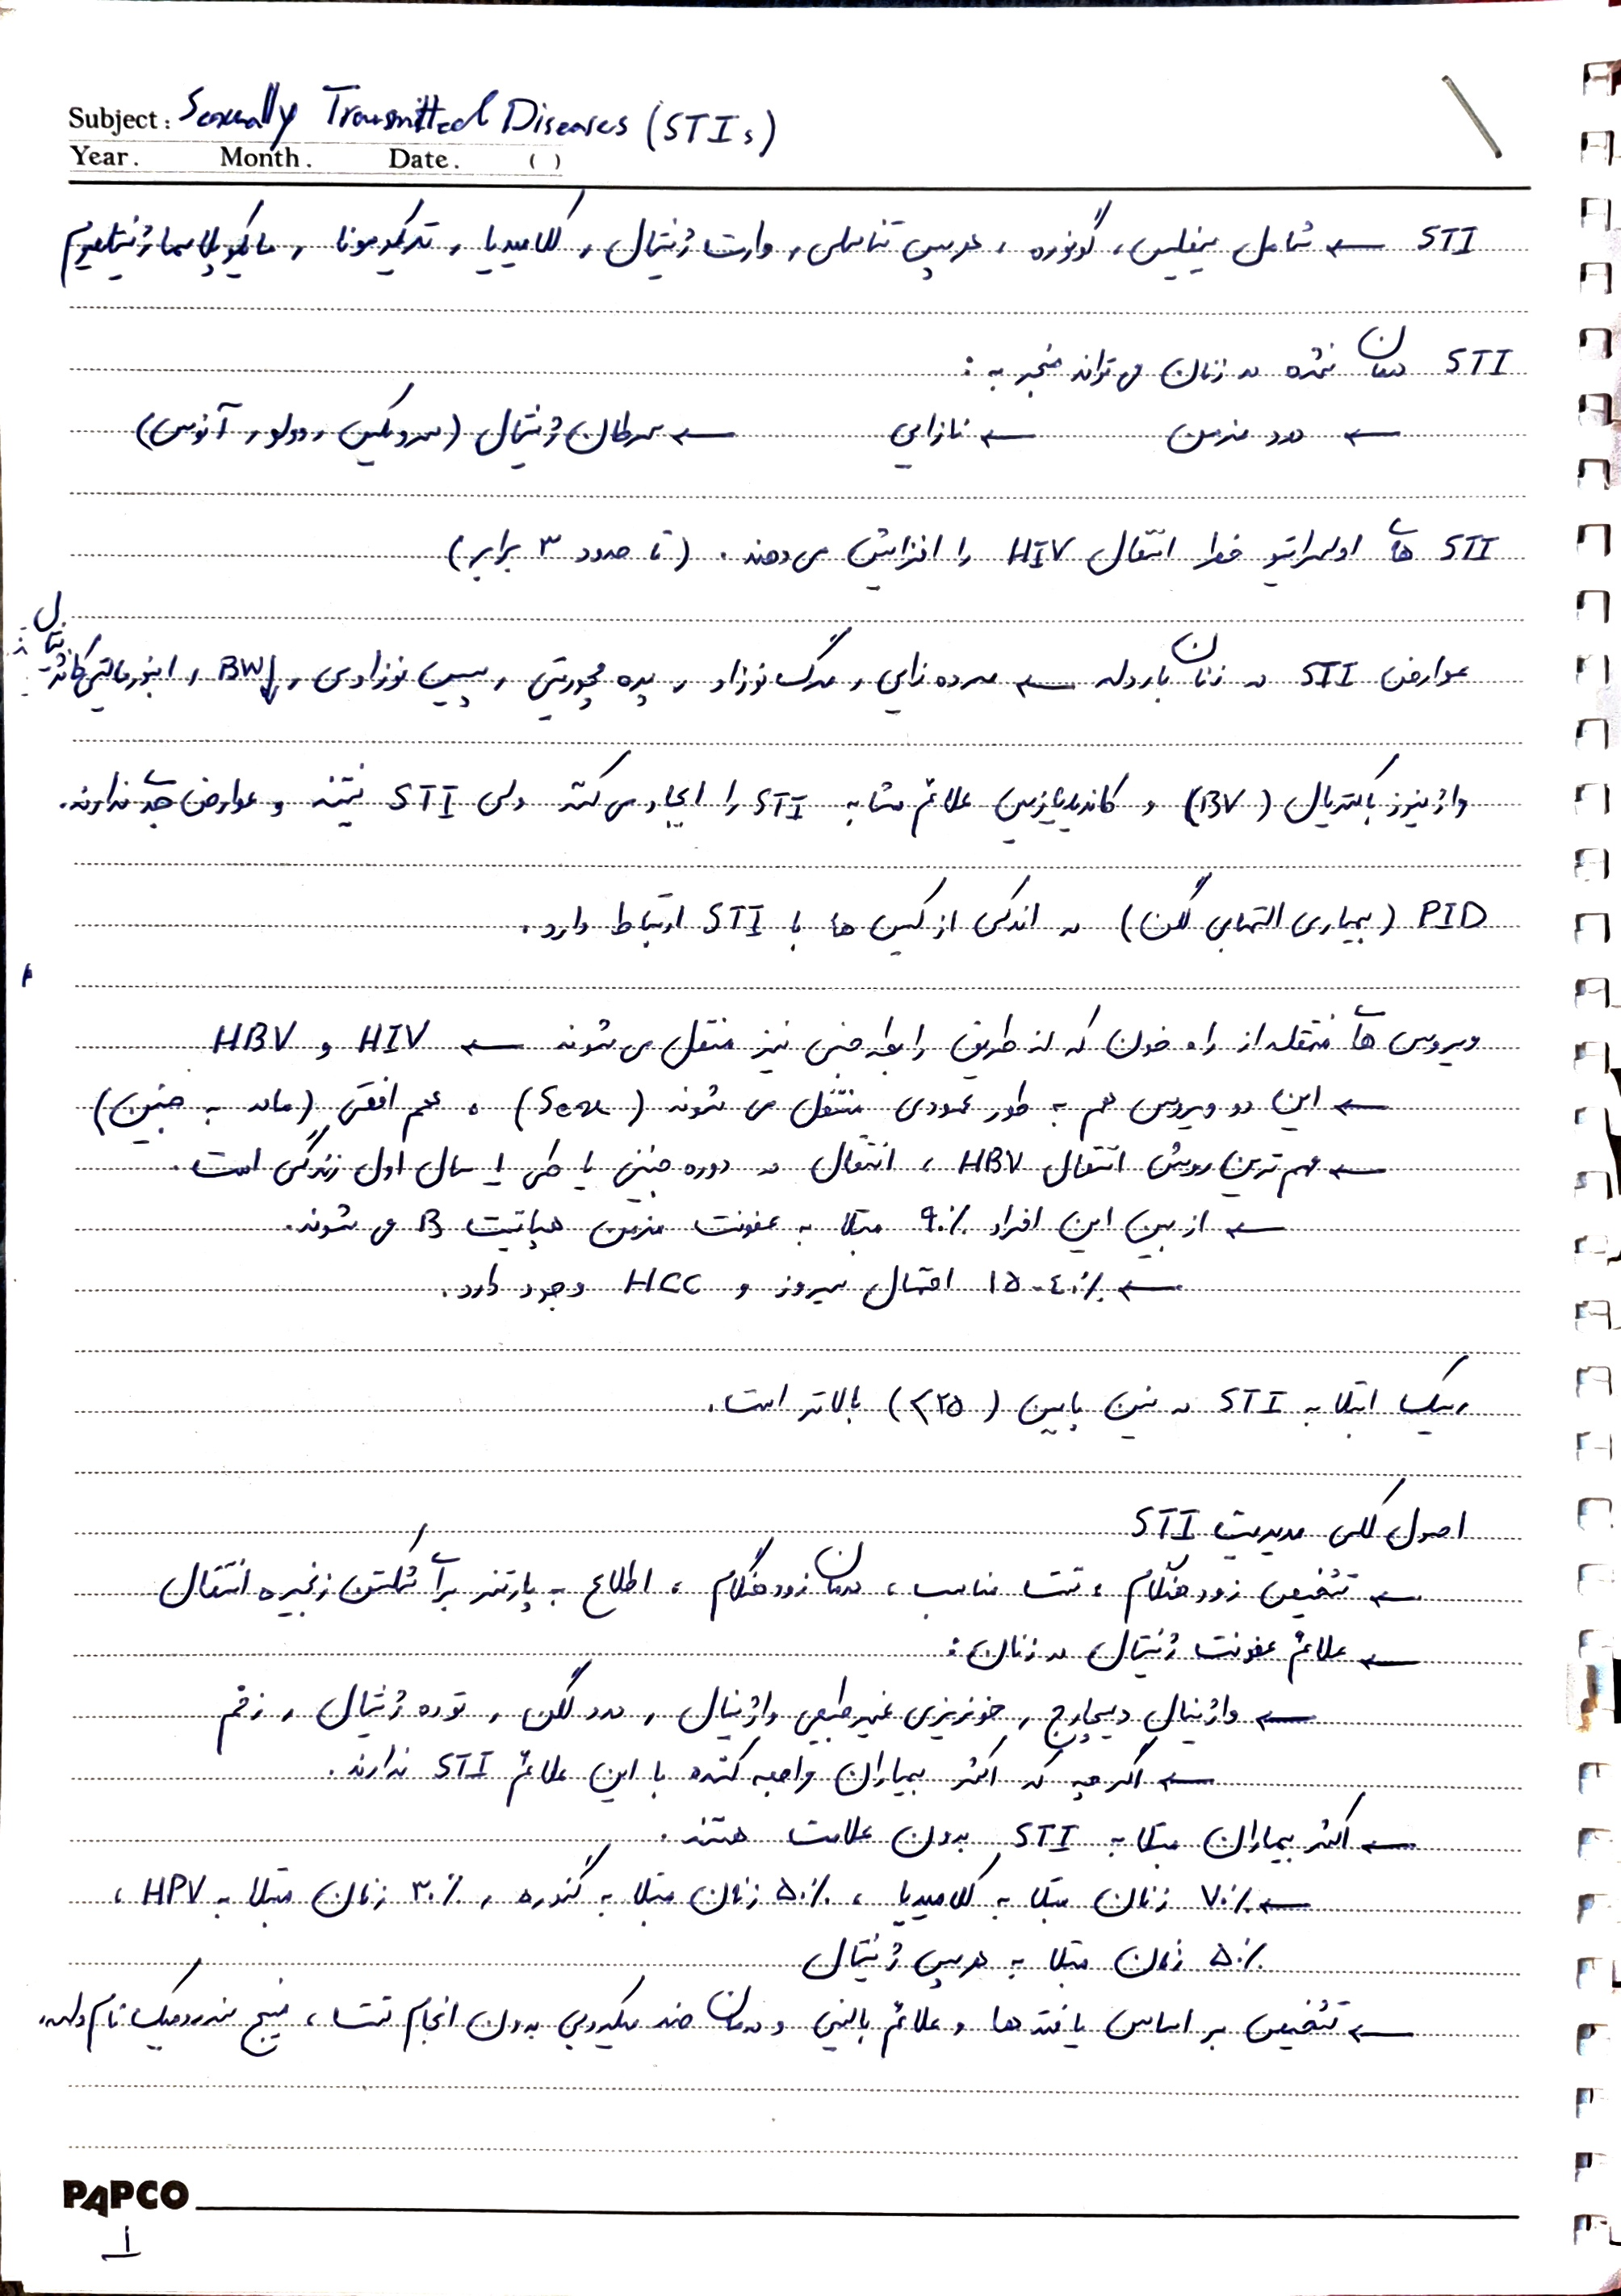
\includegraphics[width=\textwidth,height=0.86\textheight,keepaspectratio]{images/pic01.jpg}
\end{center}
\clearpage
\begin{center}
\textbf{تصویر 2}\par
\lr{\detokenize{20261011_121038628.jpg}}\par
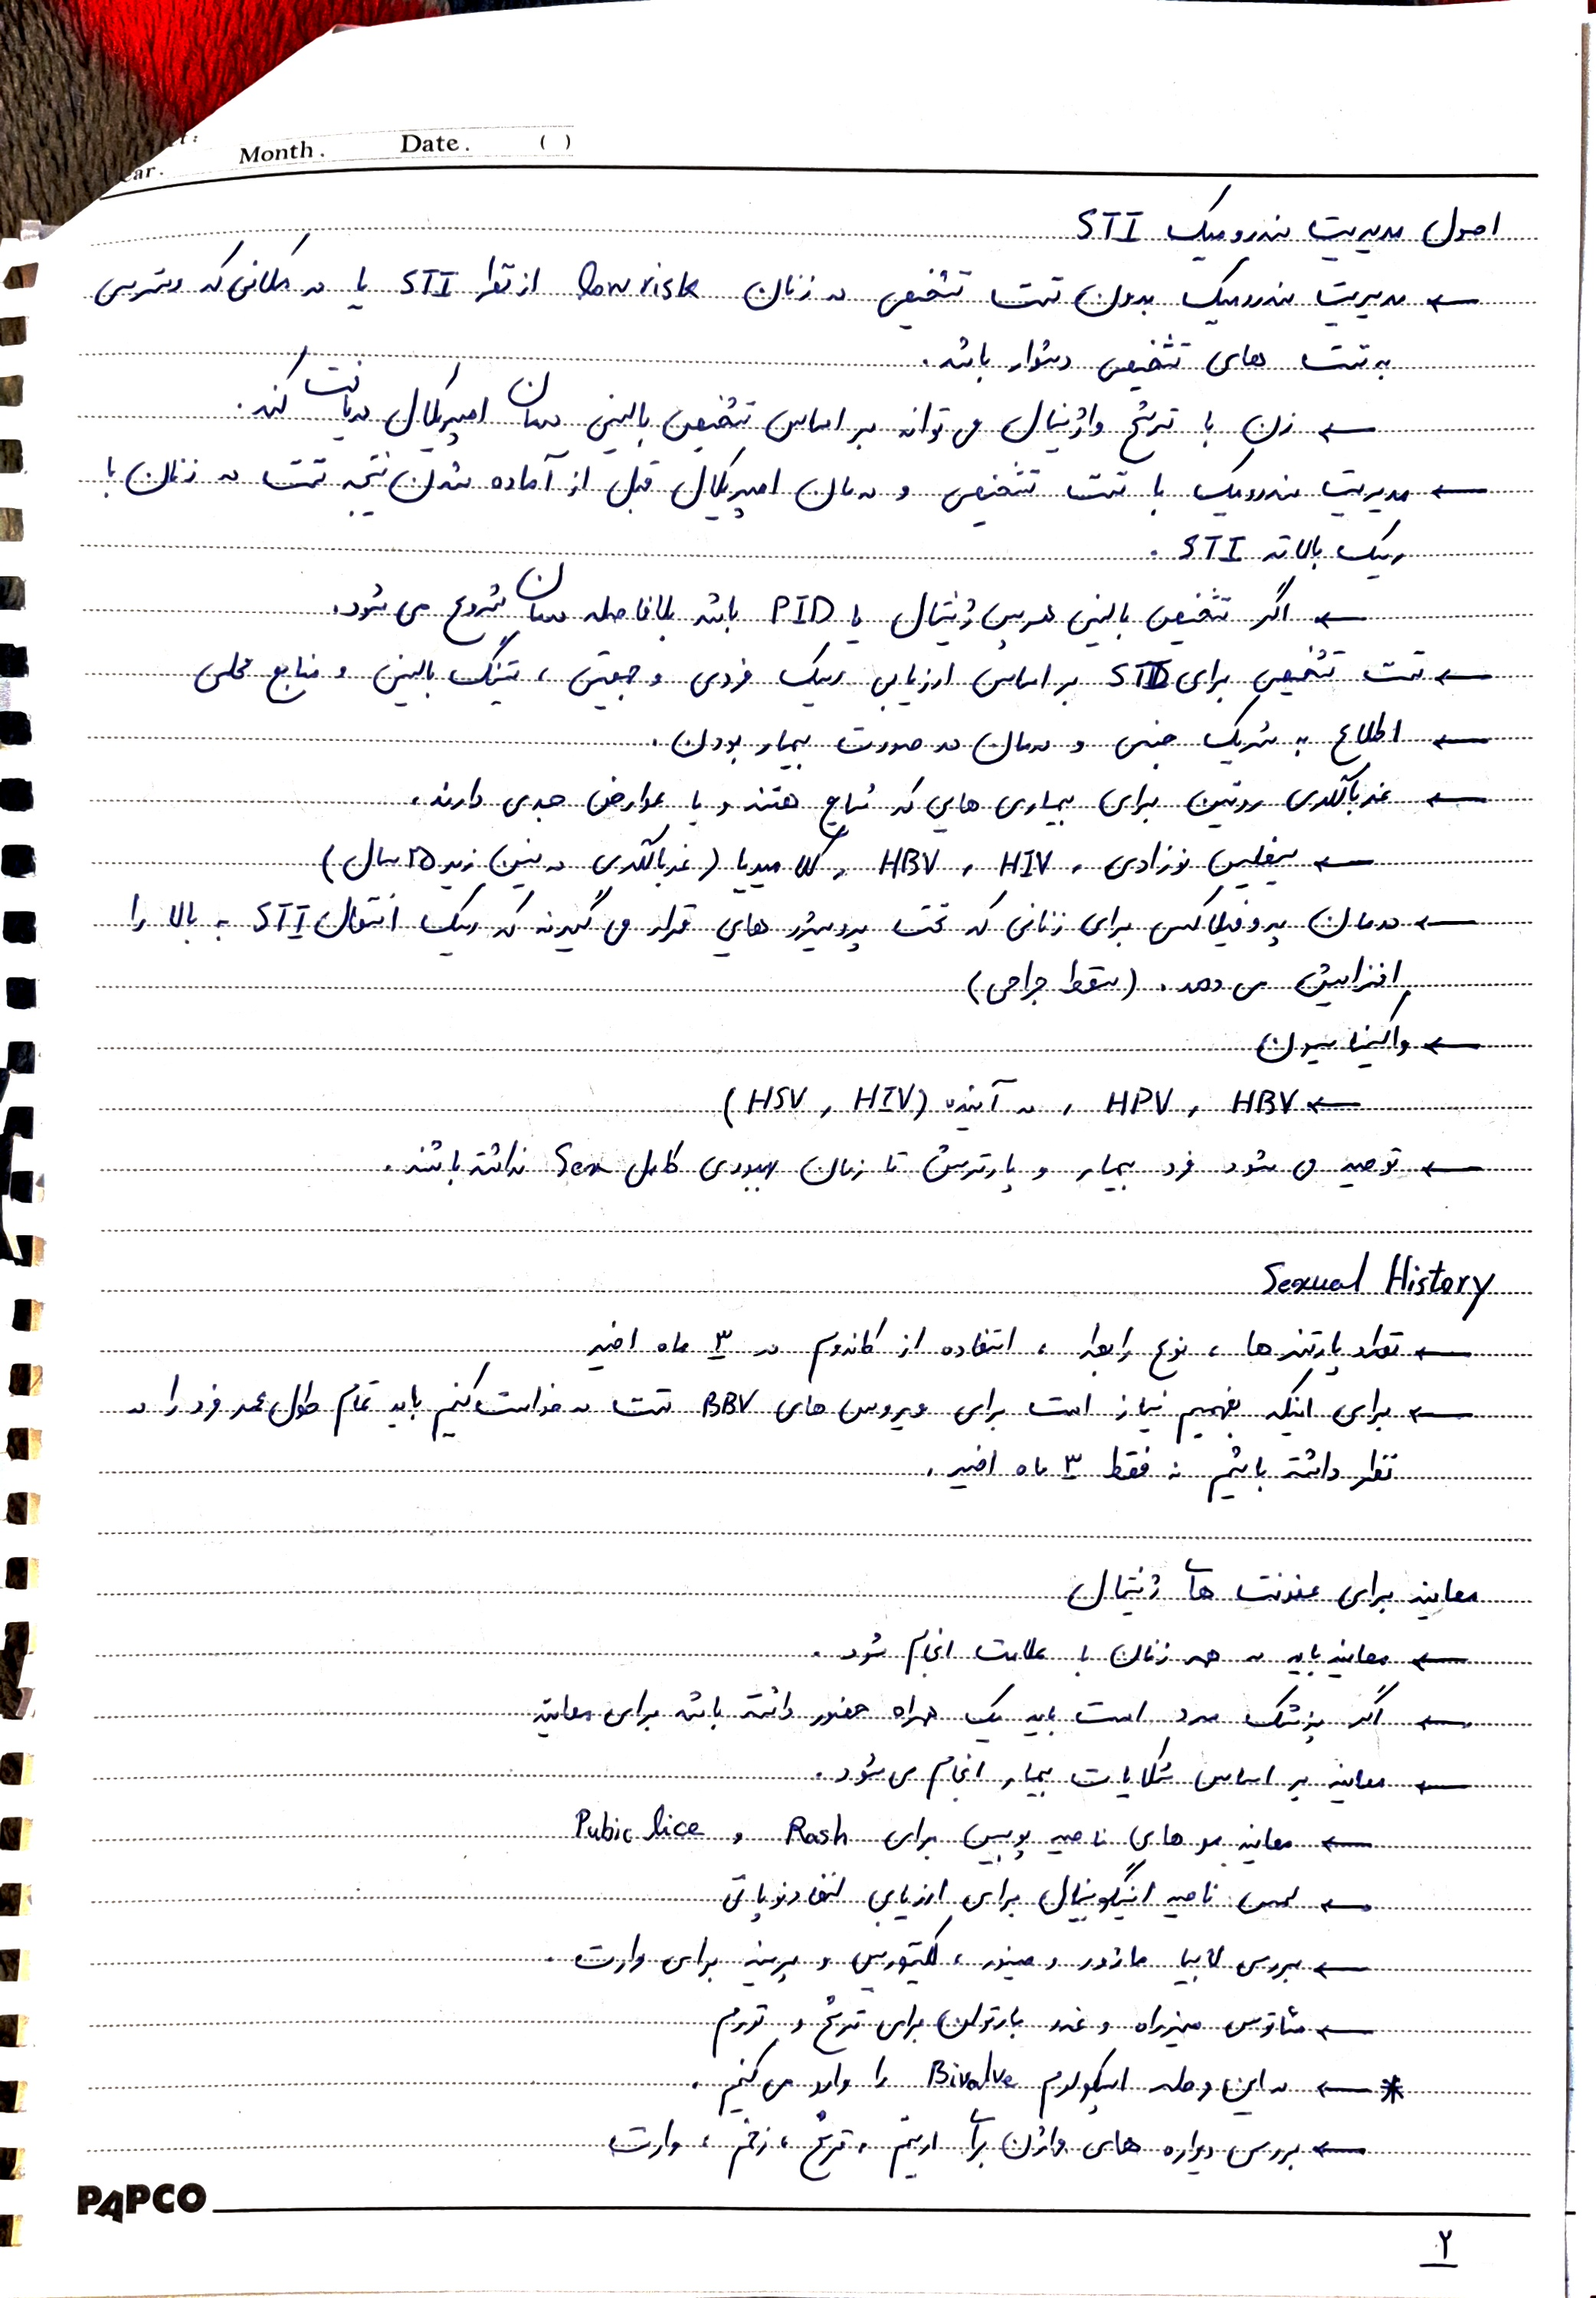
\includegraphics[width=\textwidth,height=0.86\textheight,keepaspectratio]{images/pic02.jpg}
\end{center}
\clearpage
\begin{center}
\textbf{تصویر 3}\par
\lr{\detokenize{20261011_121046667.jpg}}\par
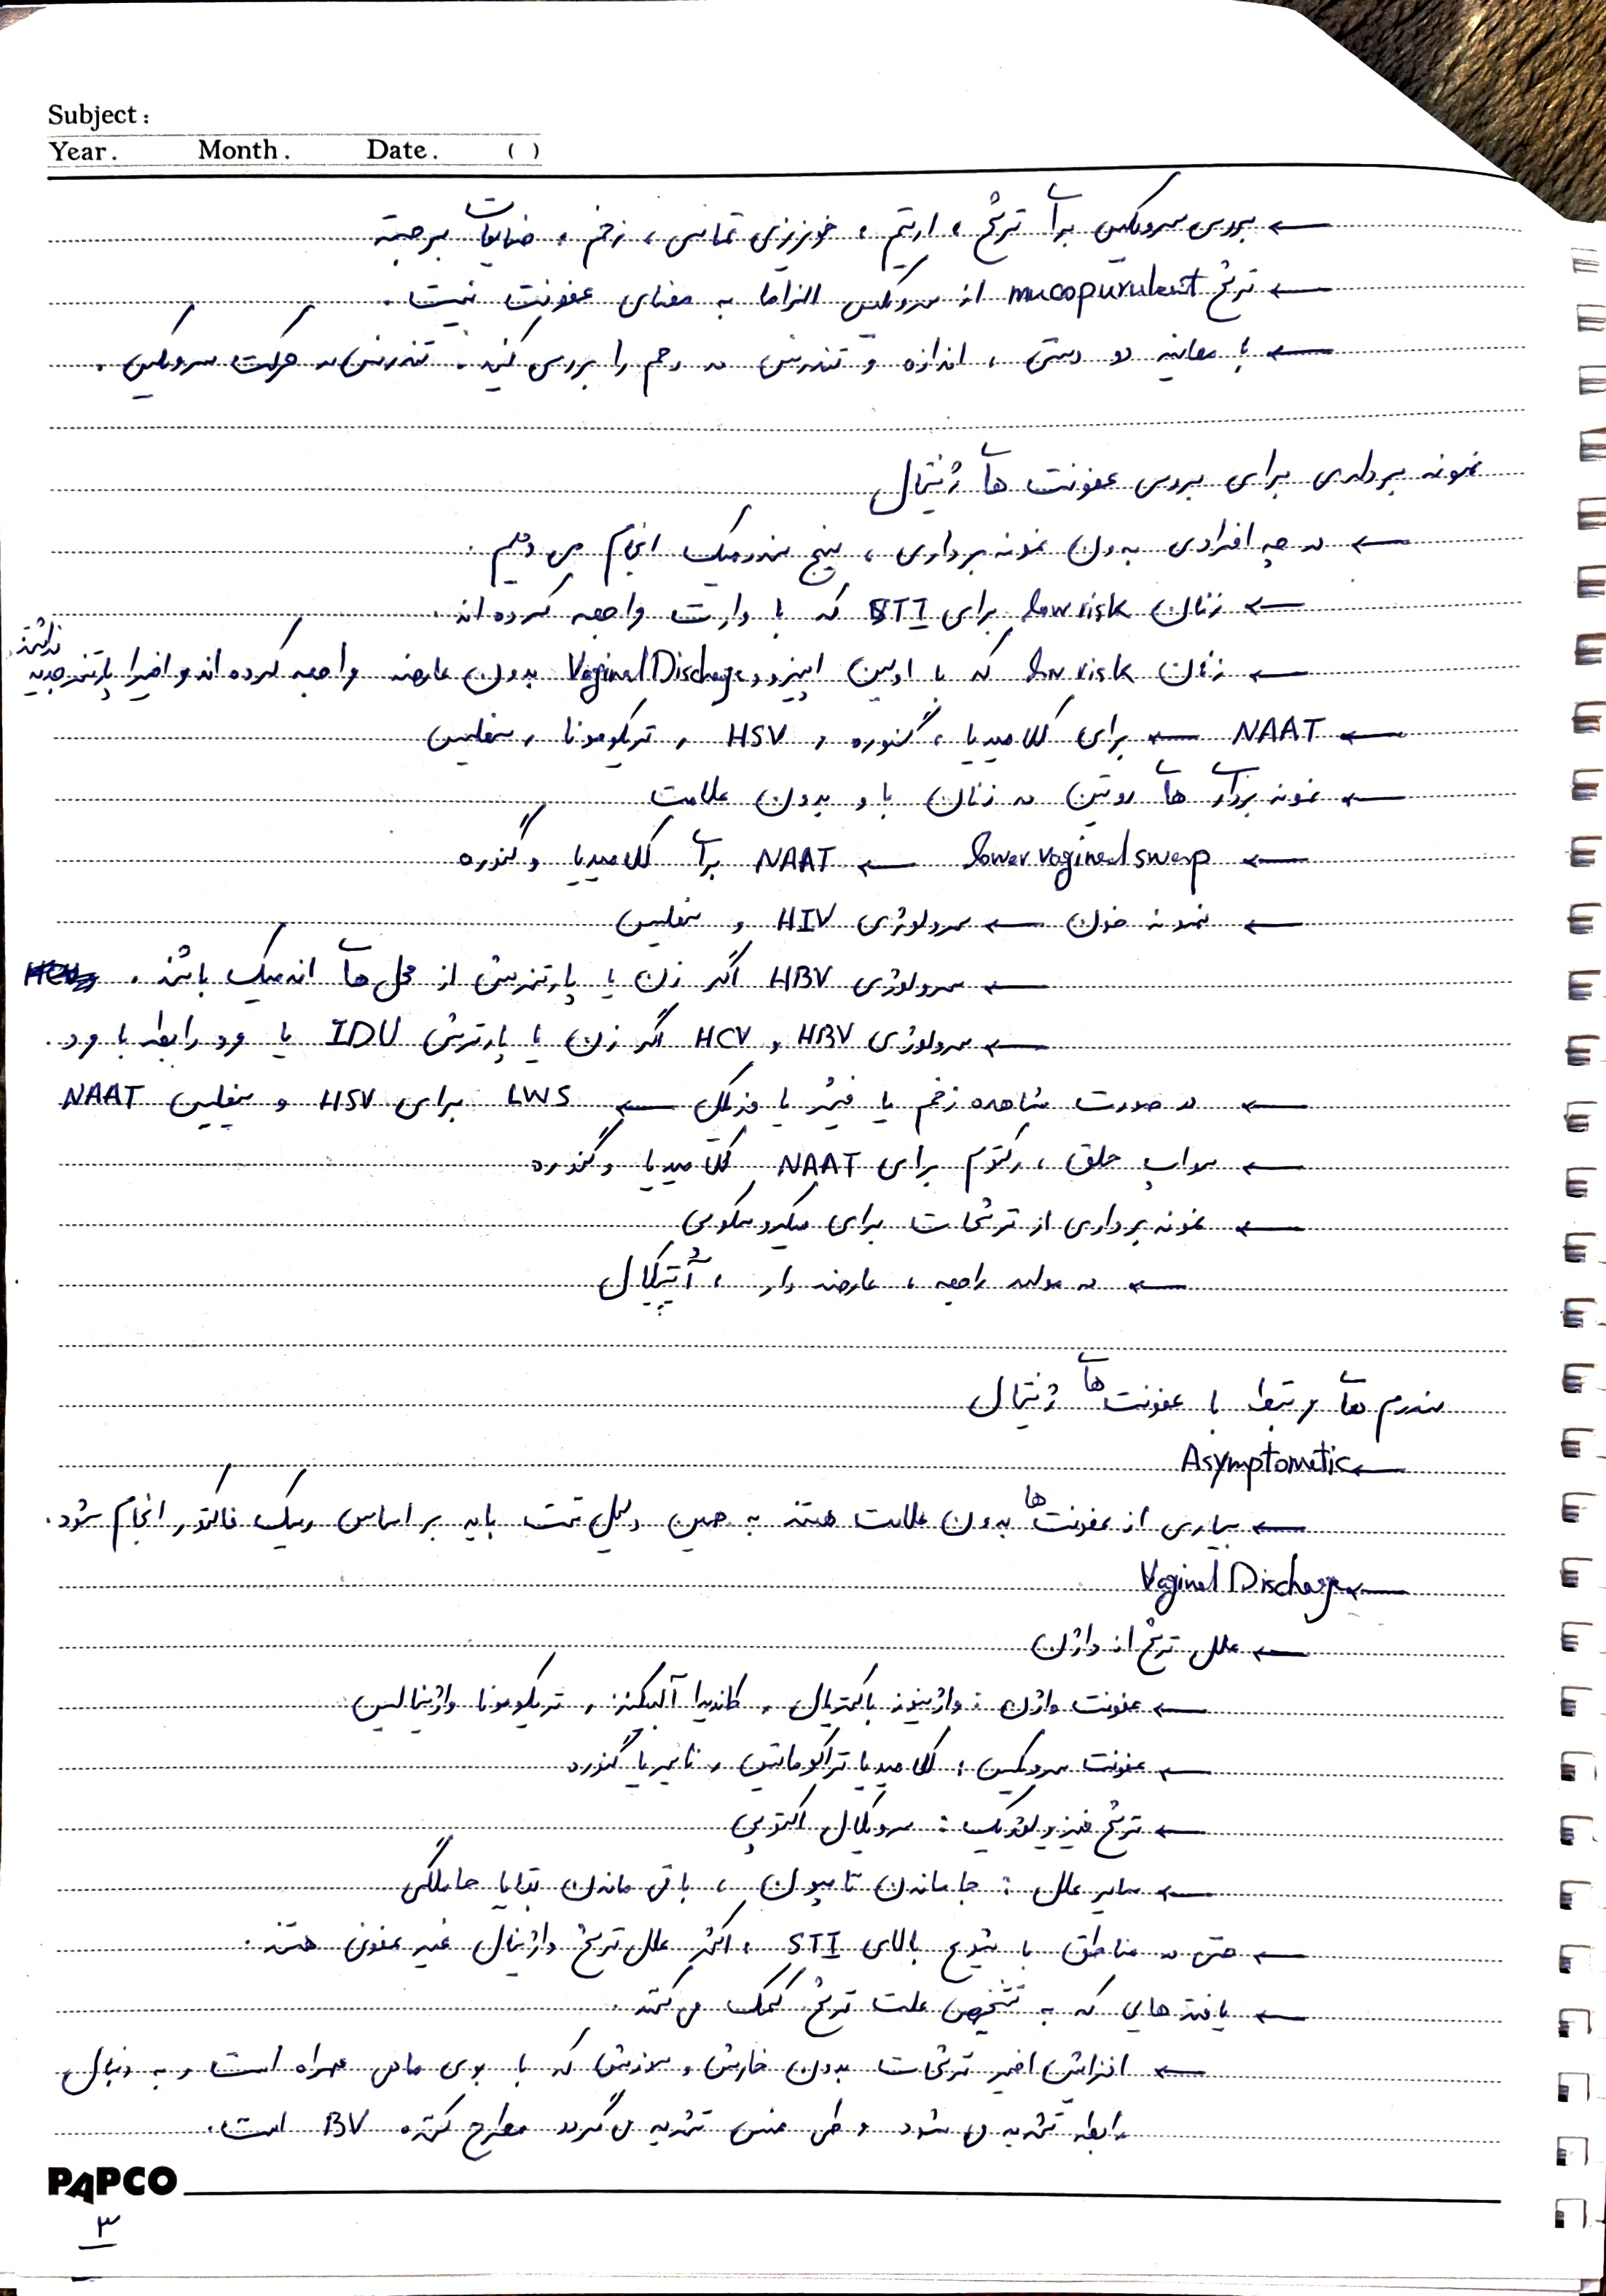
\includegraphics[width=\textwidth,height=0.86\textheight,keepaspectratio]{images/pic03.jpg}
\end{center}
\clearpage
\begin{center}
\textbf{تصویر 4}\par
\lr{\detokenize{20261011_121058449.jpg}}\par
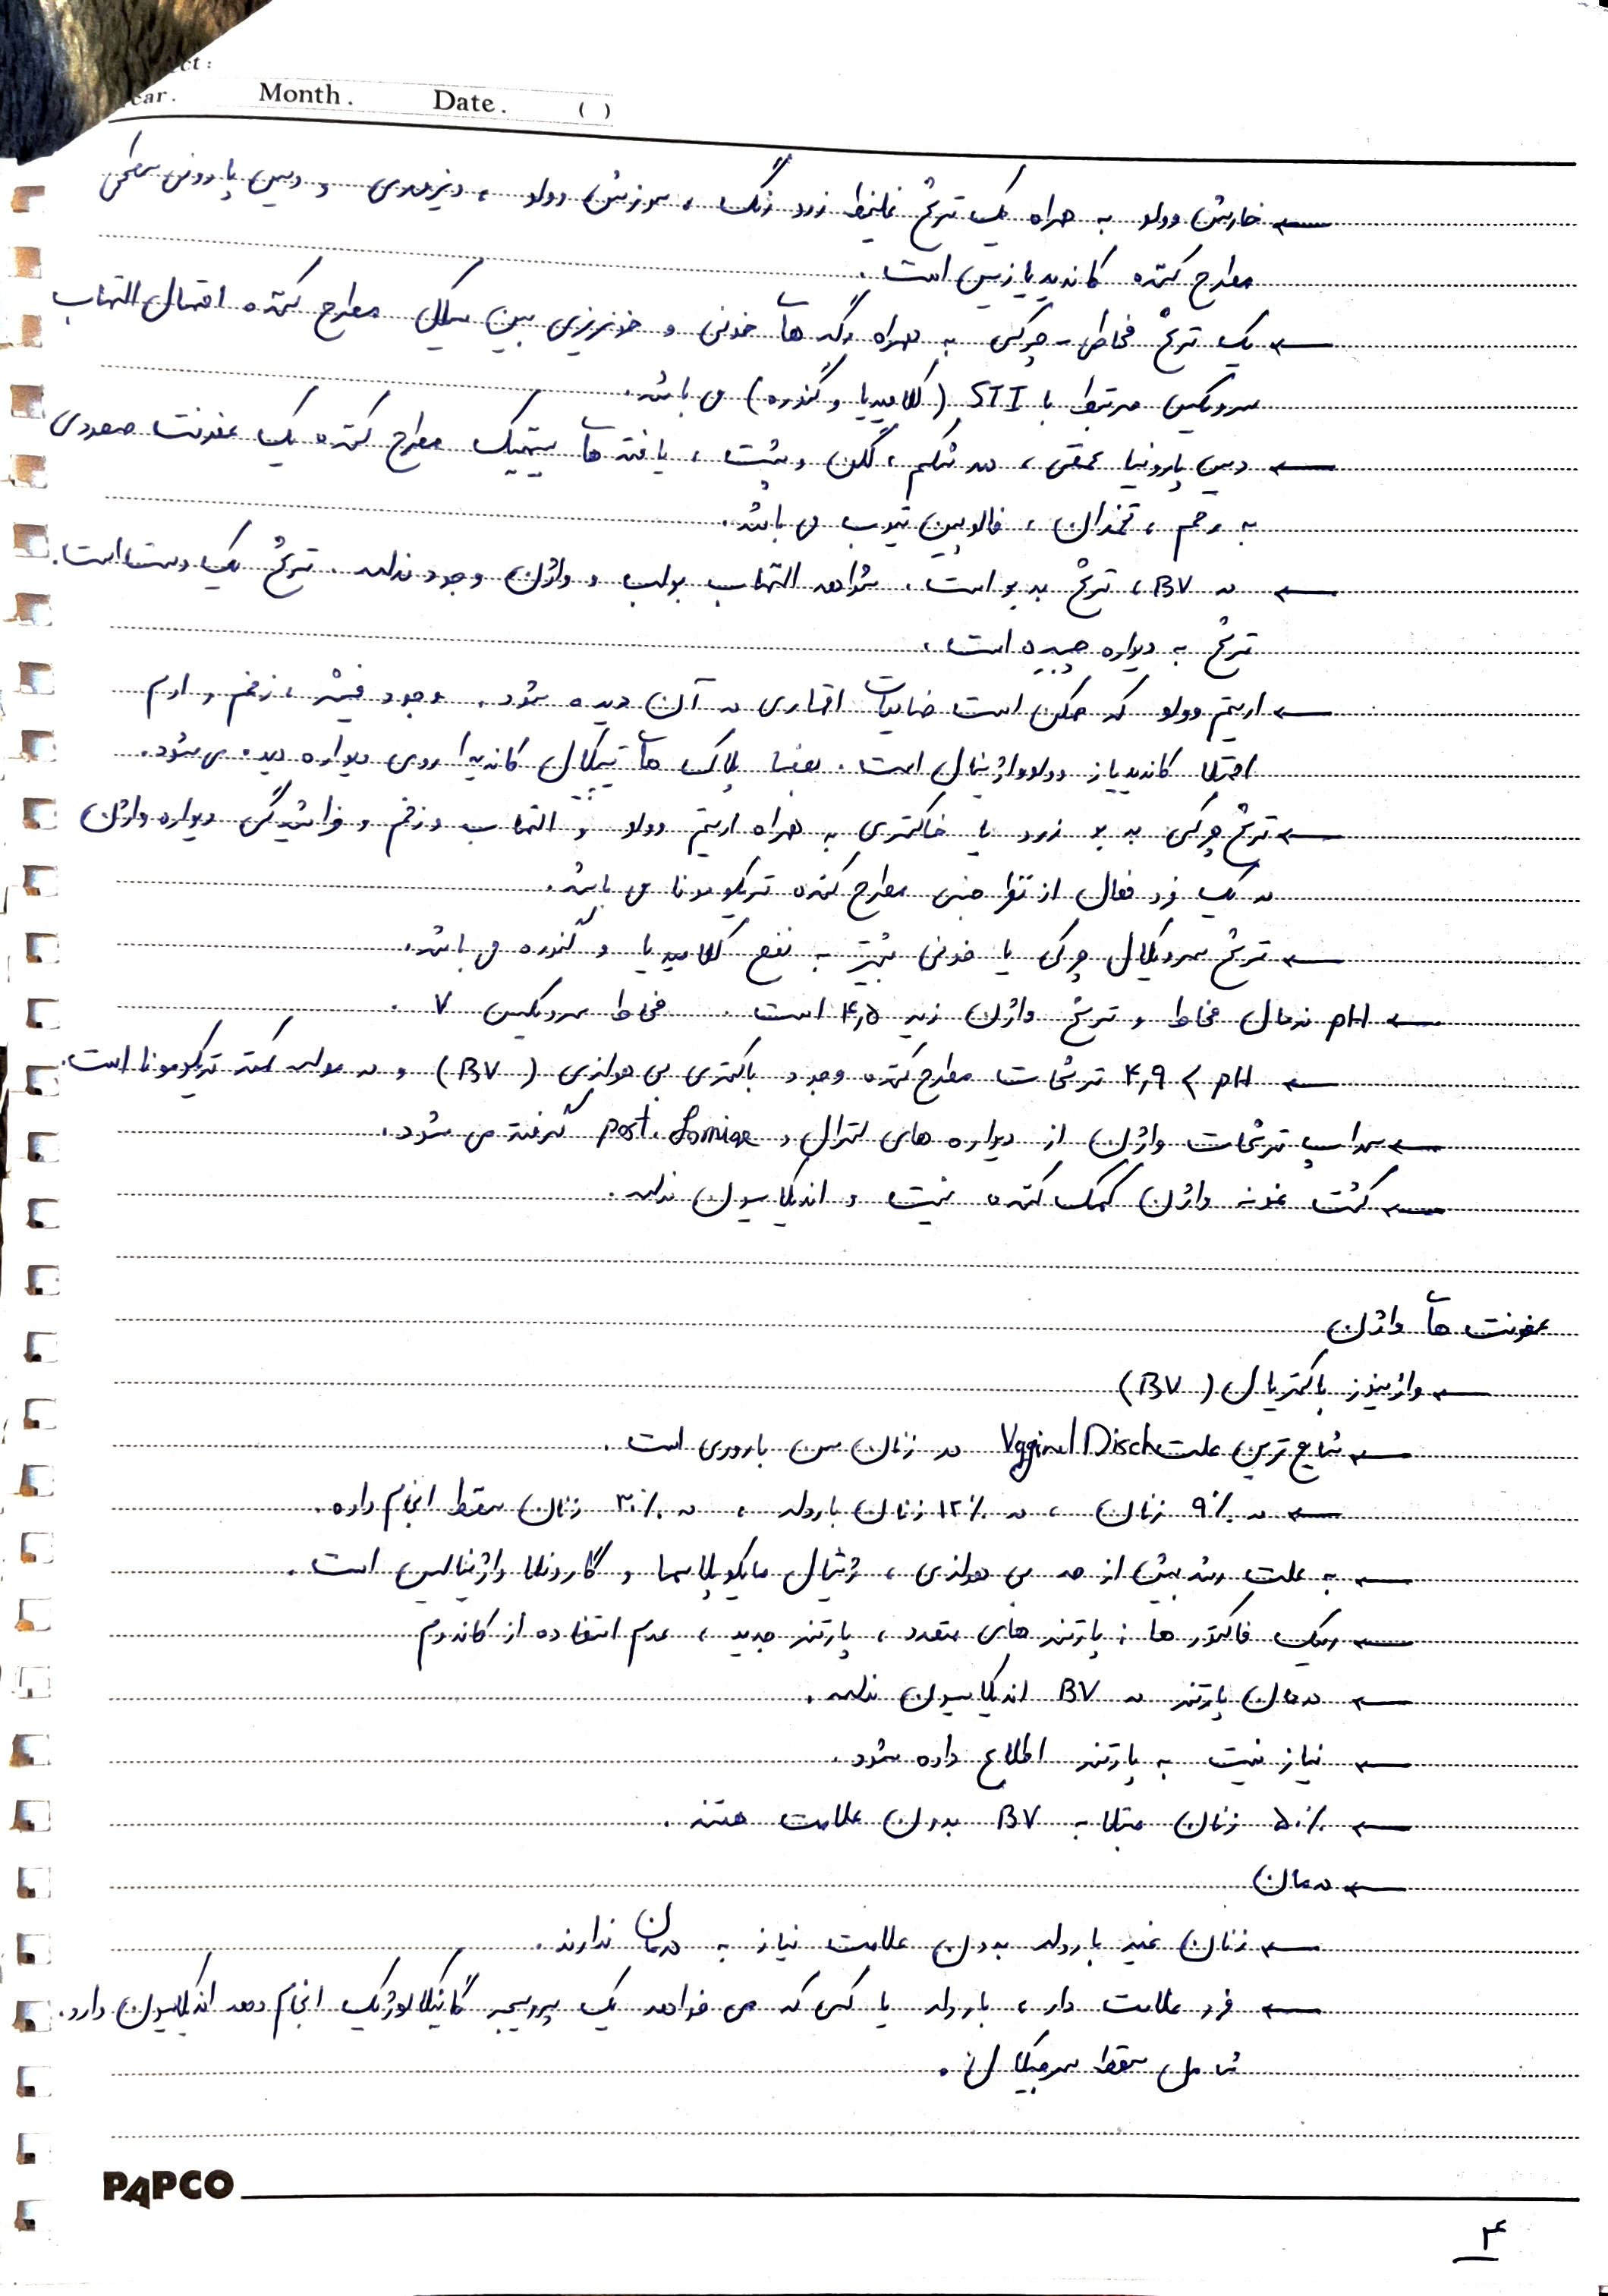
\includegraphics[width=\textwidth,height=0.86\textheight,keepaspectratio]{images/pic04.jpg}
\end{center}
\clearpage
\begin{center}
\textbf{تصویر 5}\par
\lr{\detokenize{20261011_121102894.jpg}}\par
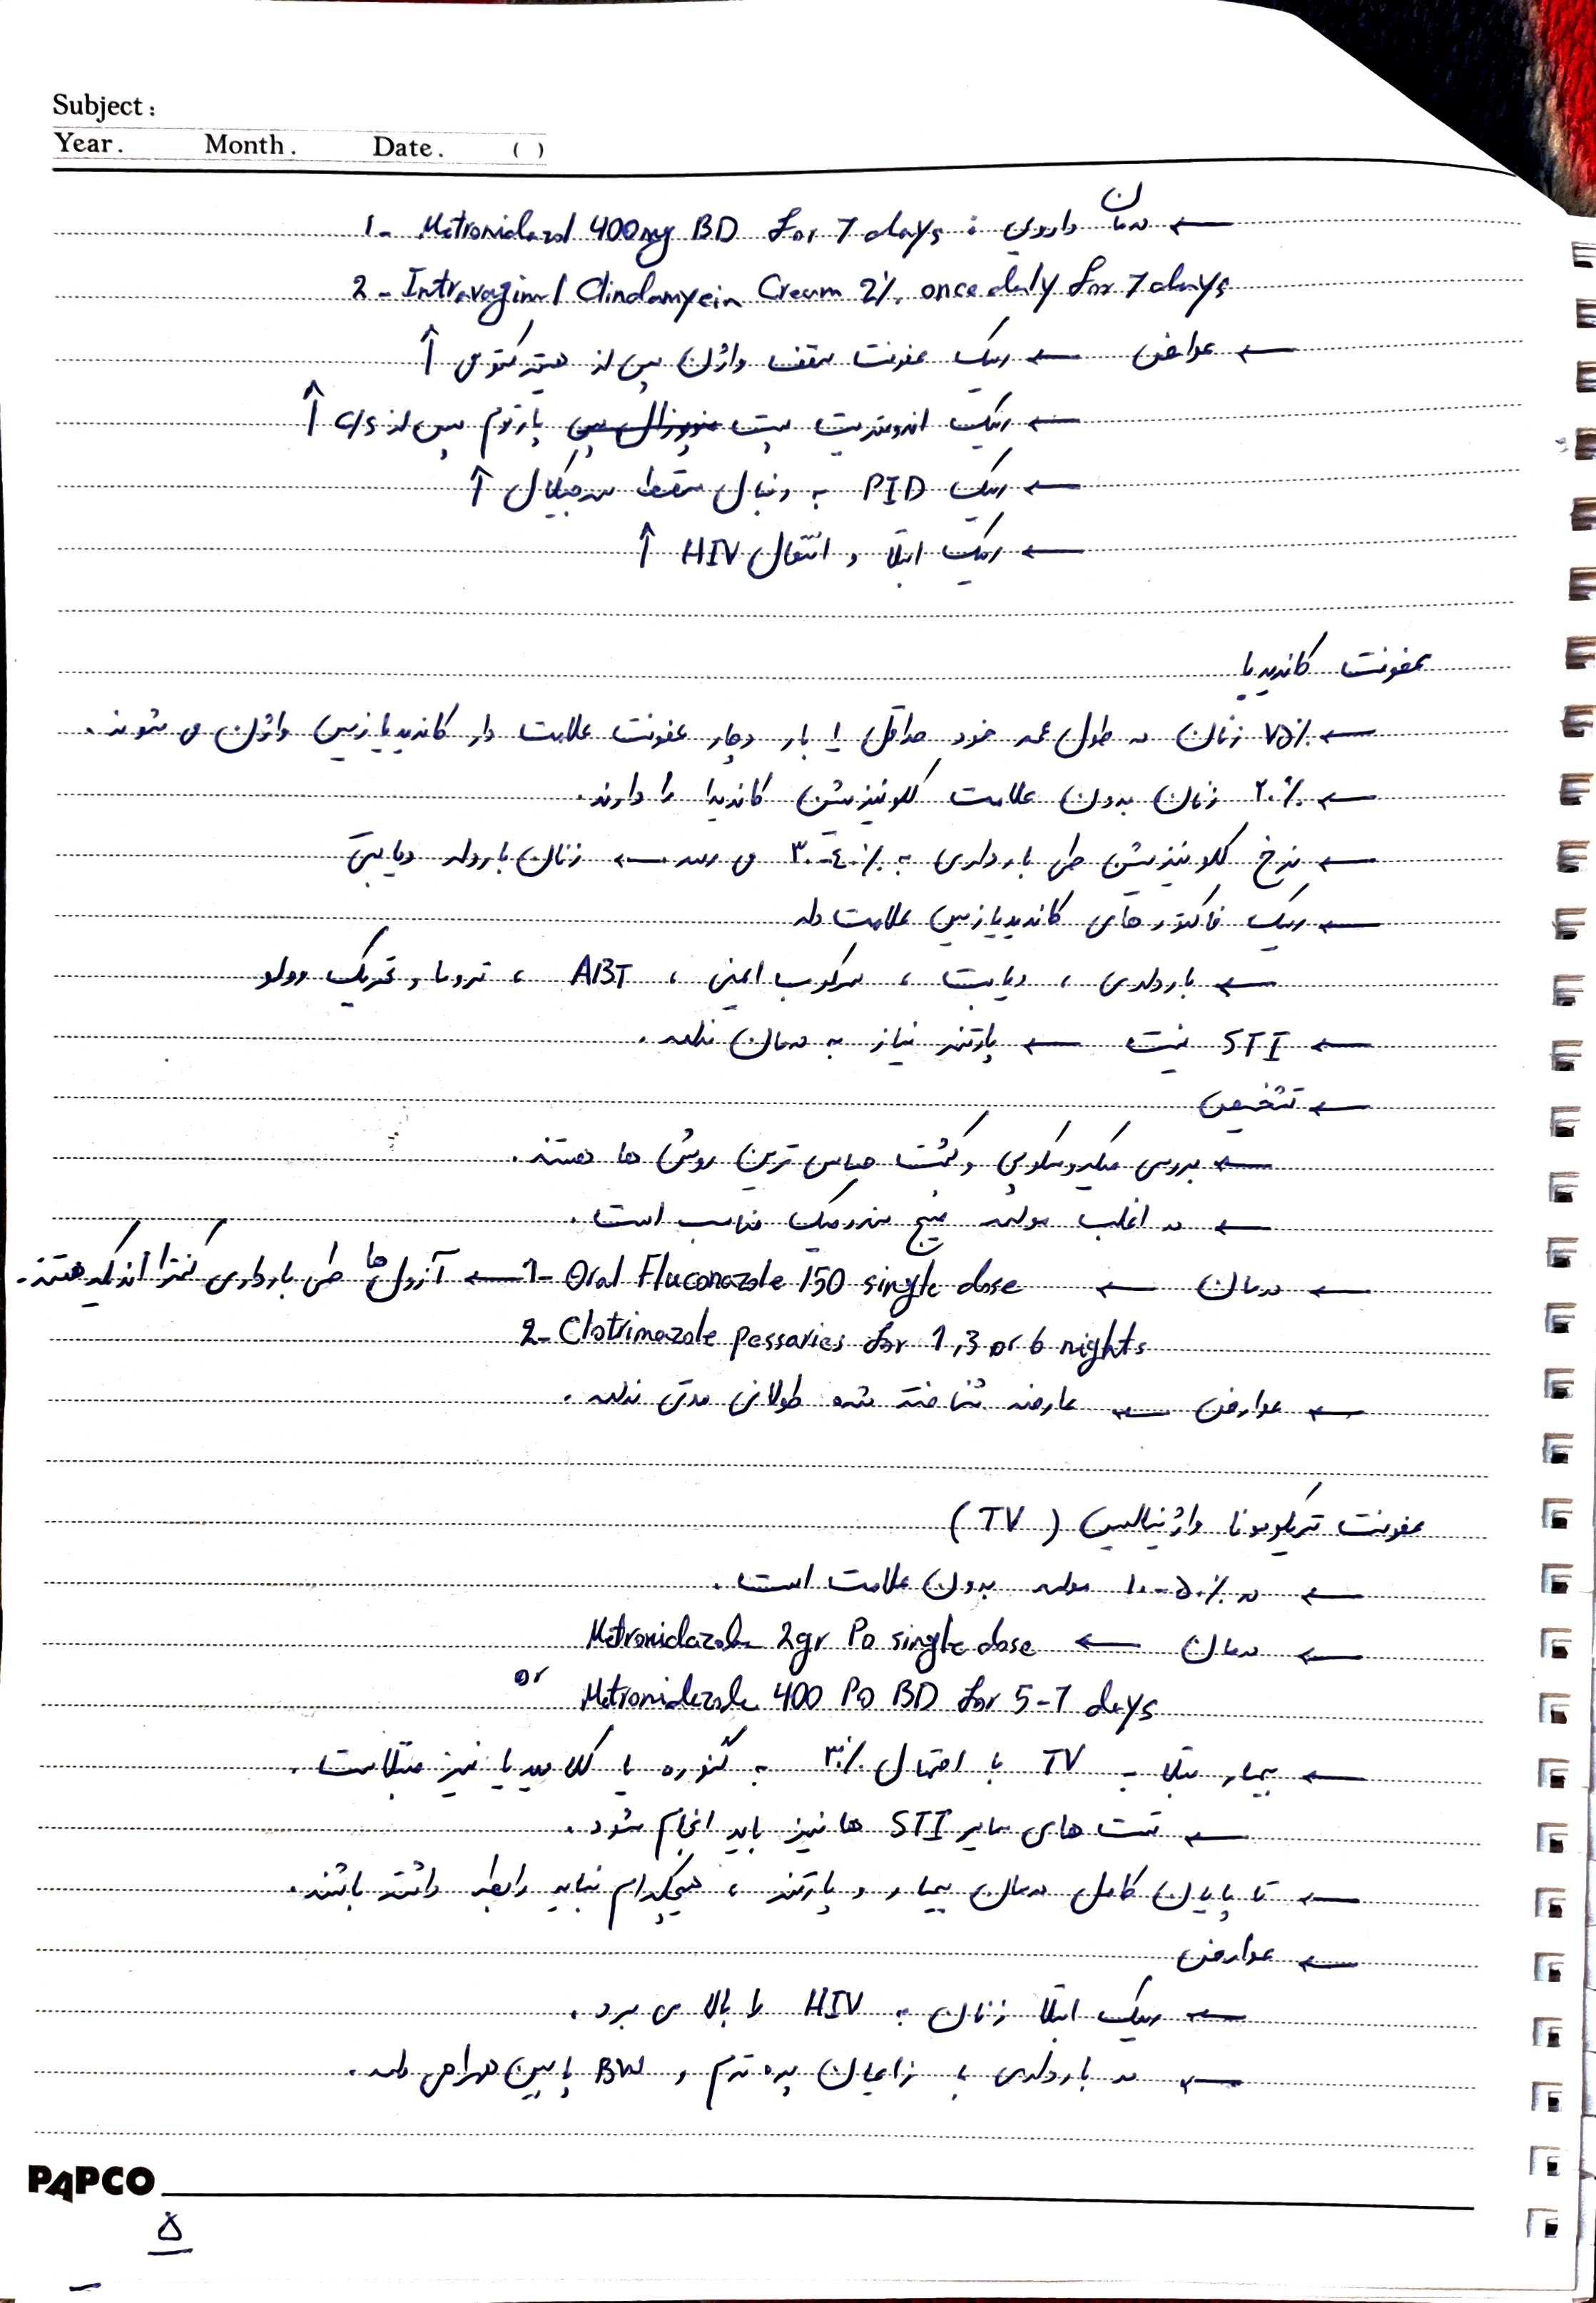
\includegraphics[width=\textwidth,height=0.86\textheight,keepaspectratio]{images/pic05.jpg}
\end{center}
\clearpage
\begin{center}
\textbf{تصویر 6}\par
\lr{\detokenize{20261011_121115043.jpg}}\par
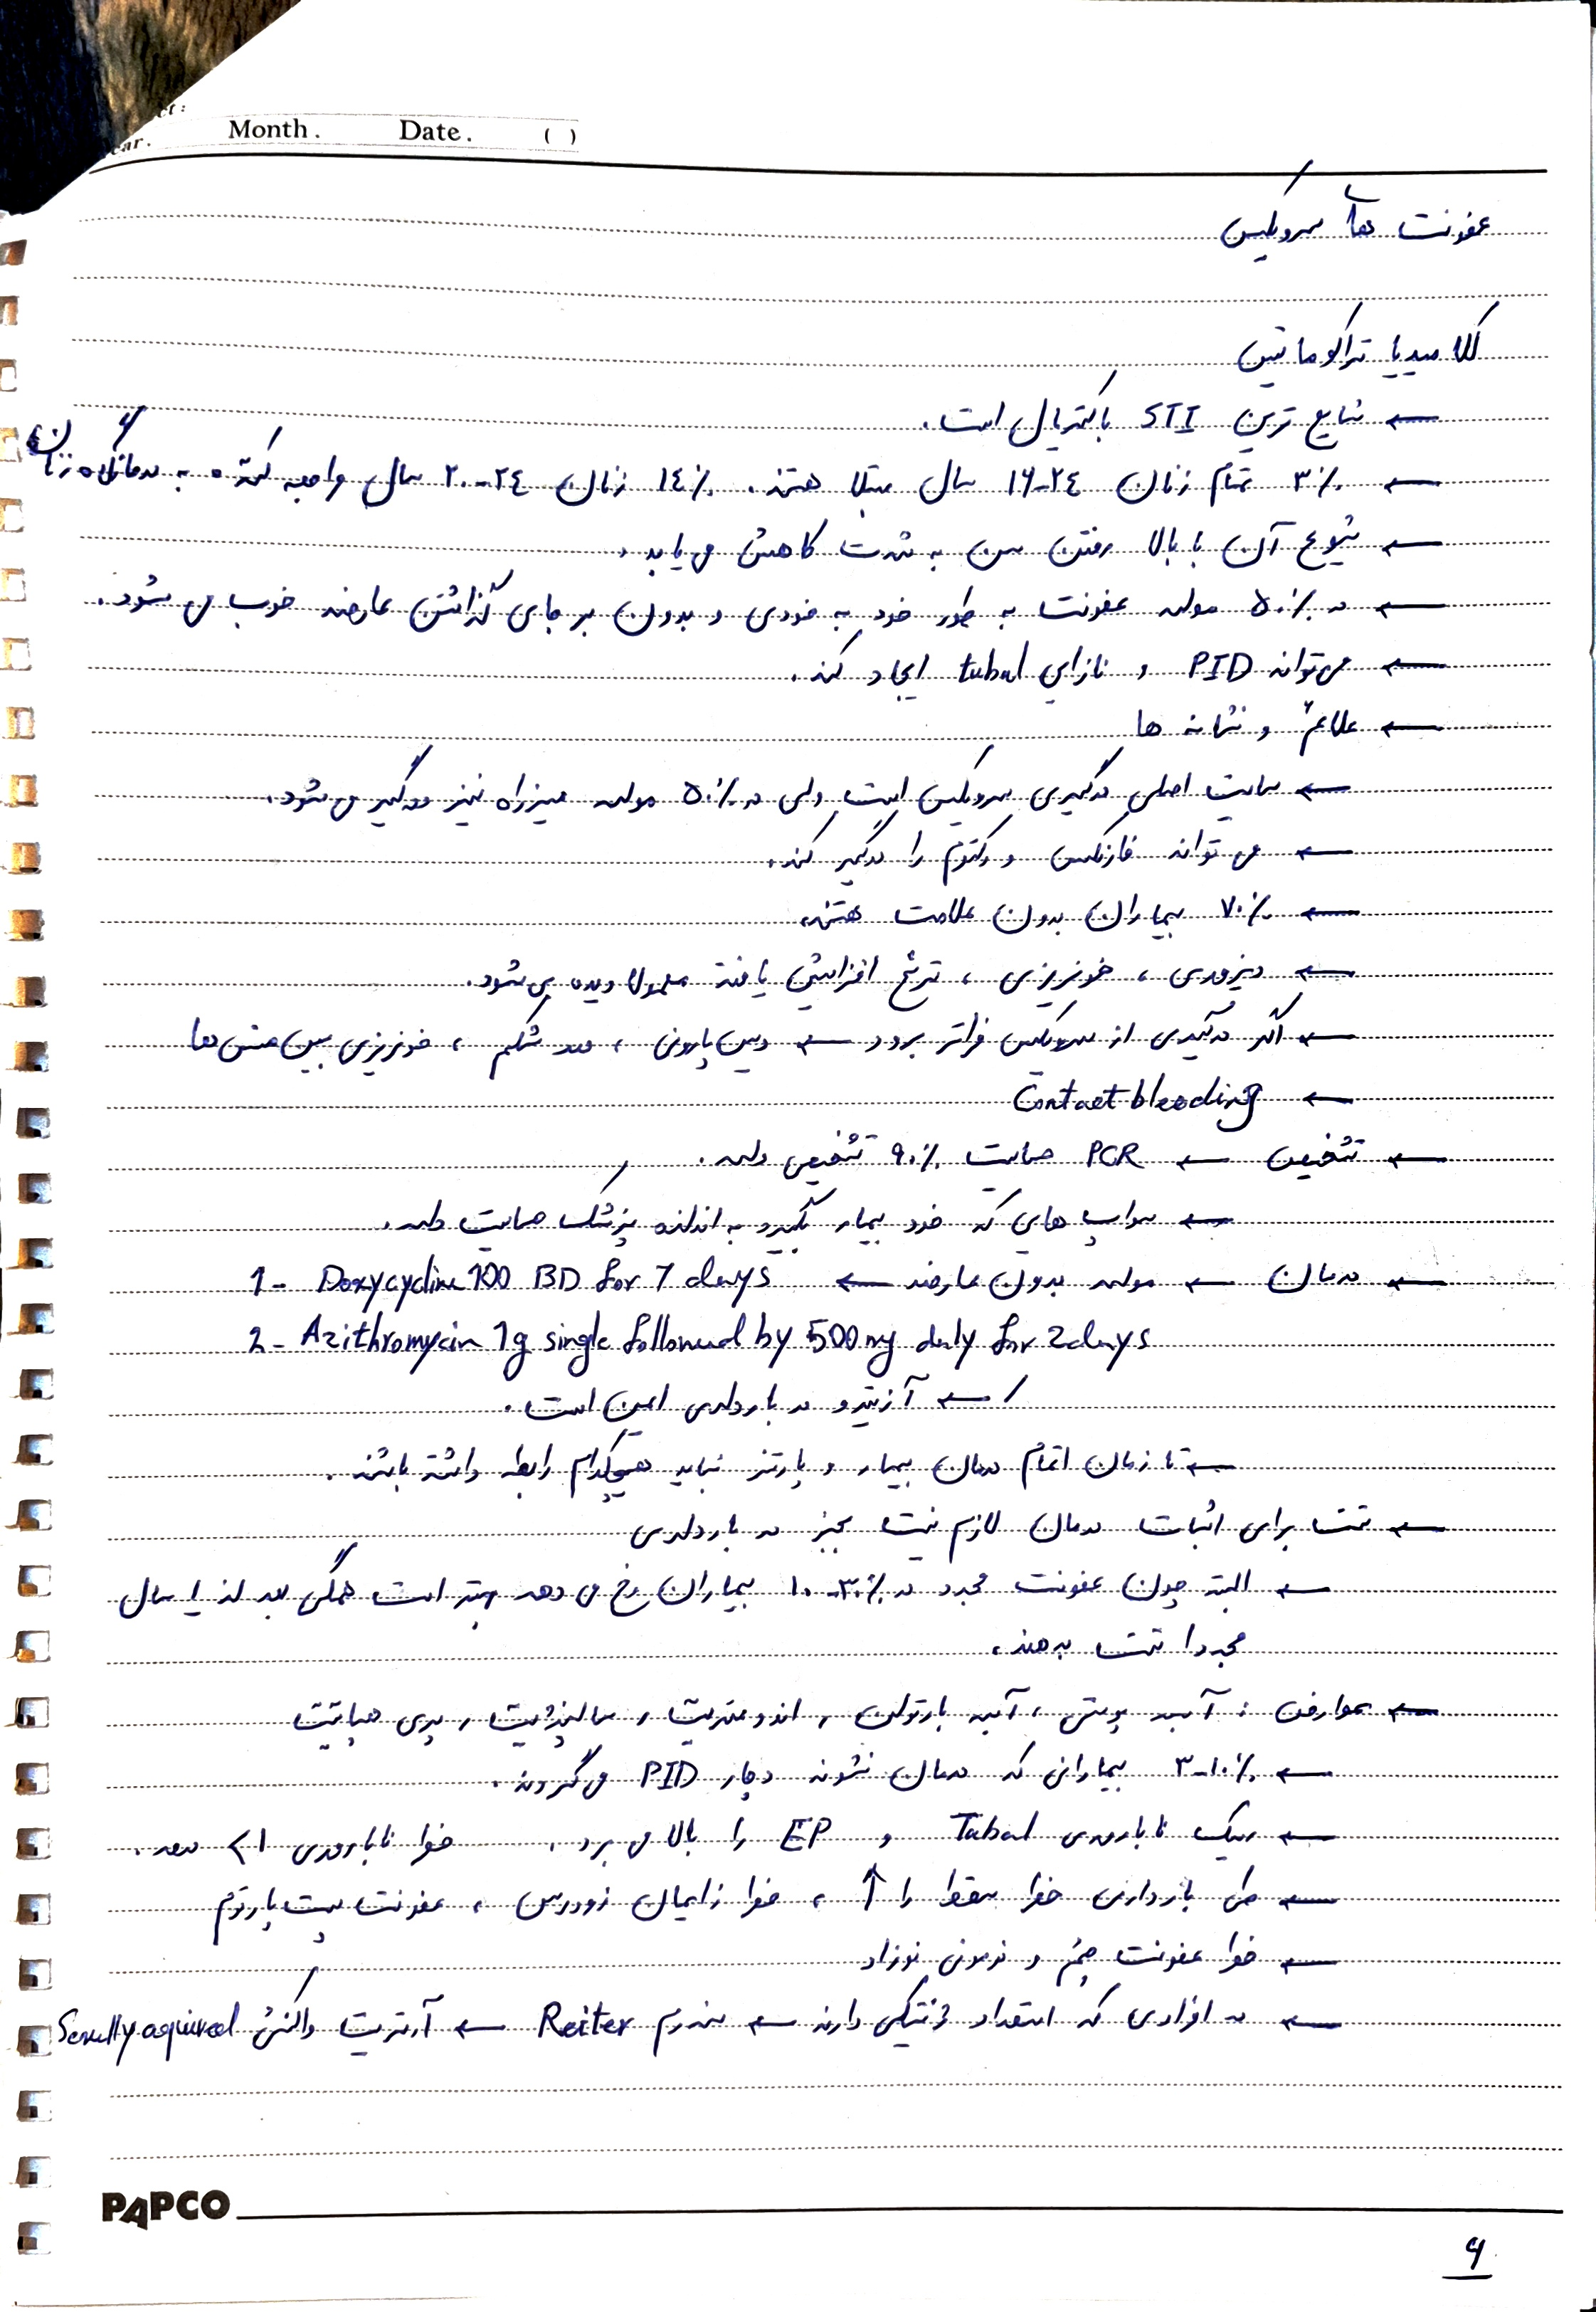
\includegraphics[width=\textwidth,height=0.86\textheight,keepaspectratio]{images/pic06.jpg}
\end{center}
\clearpage
\begin{center}
\textbf{تصویر 7}\par
\lr{\detokenize{20261011_121119559.jpg}}\par
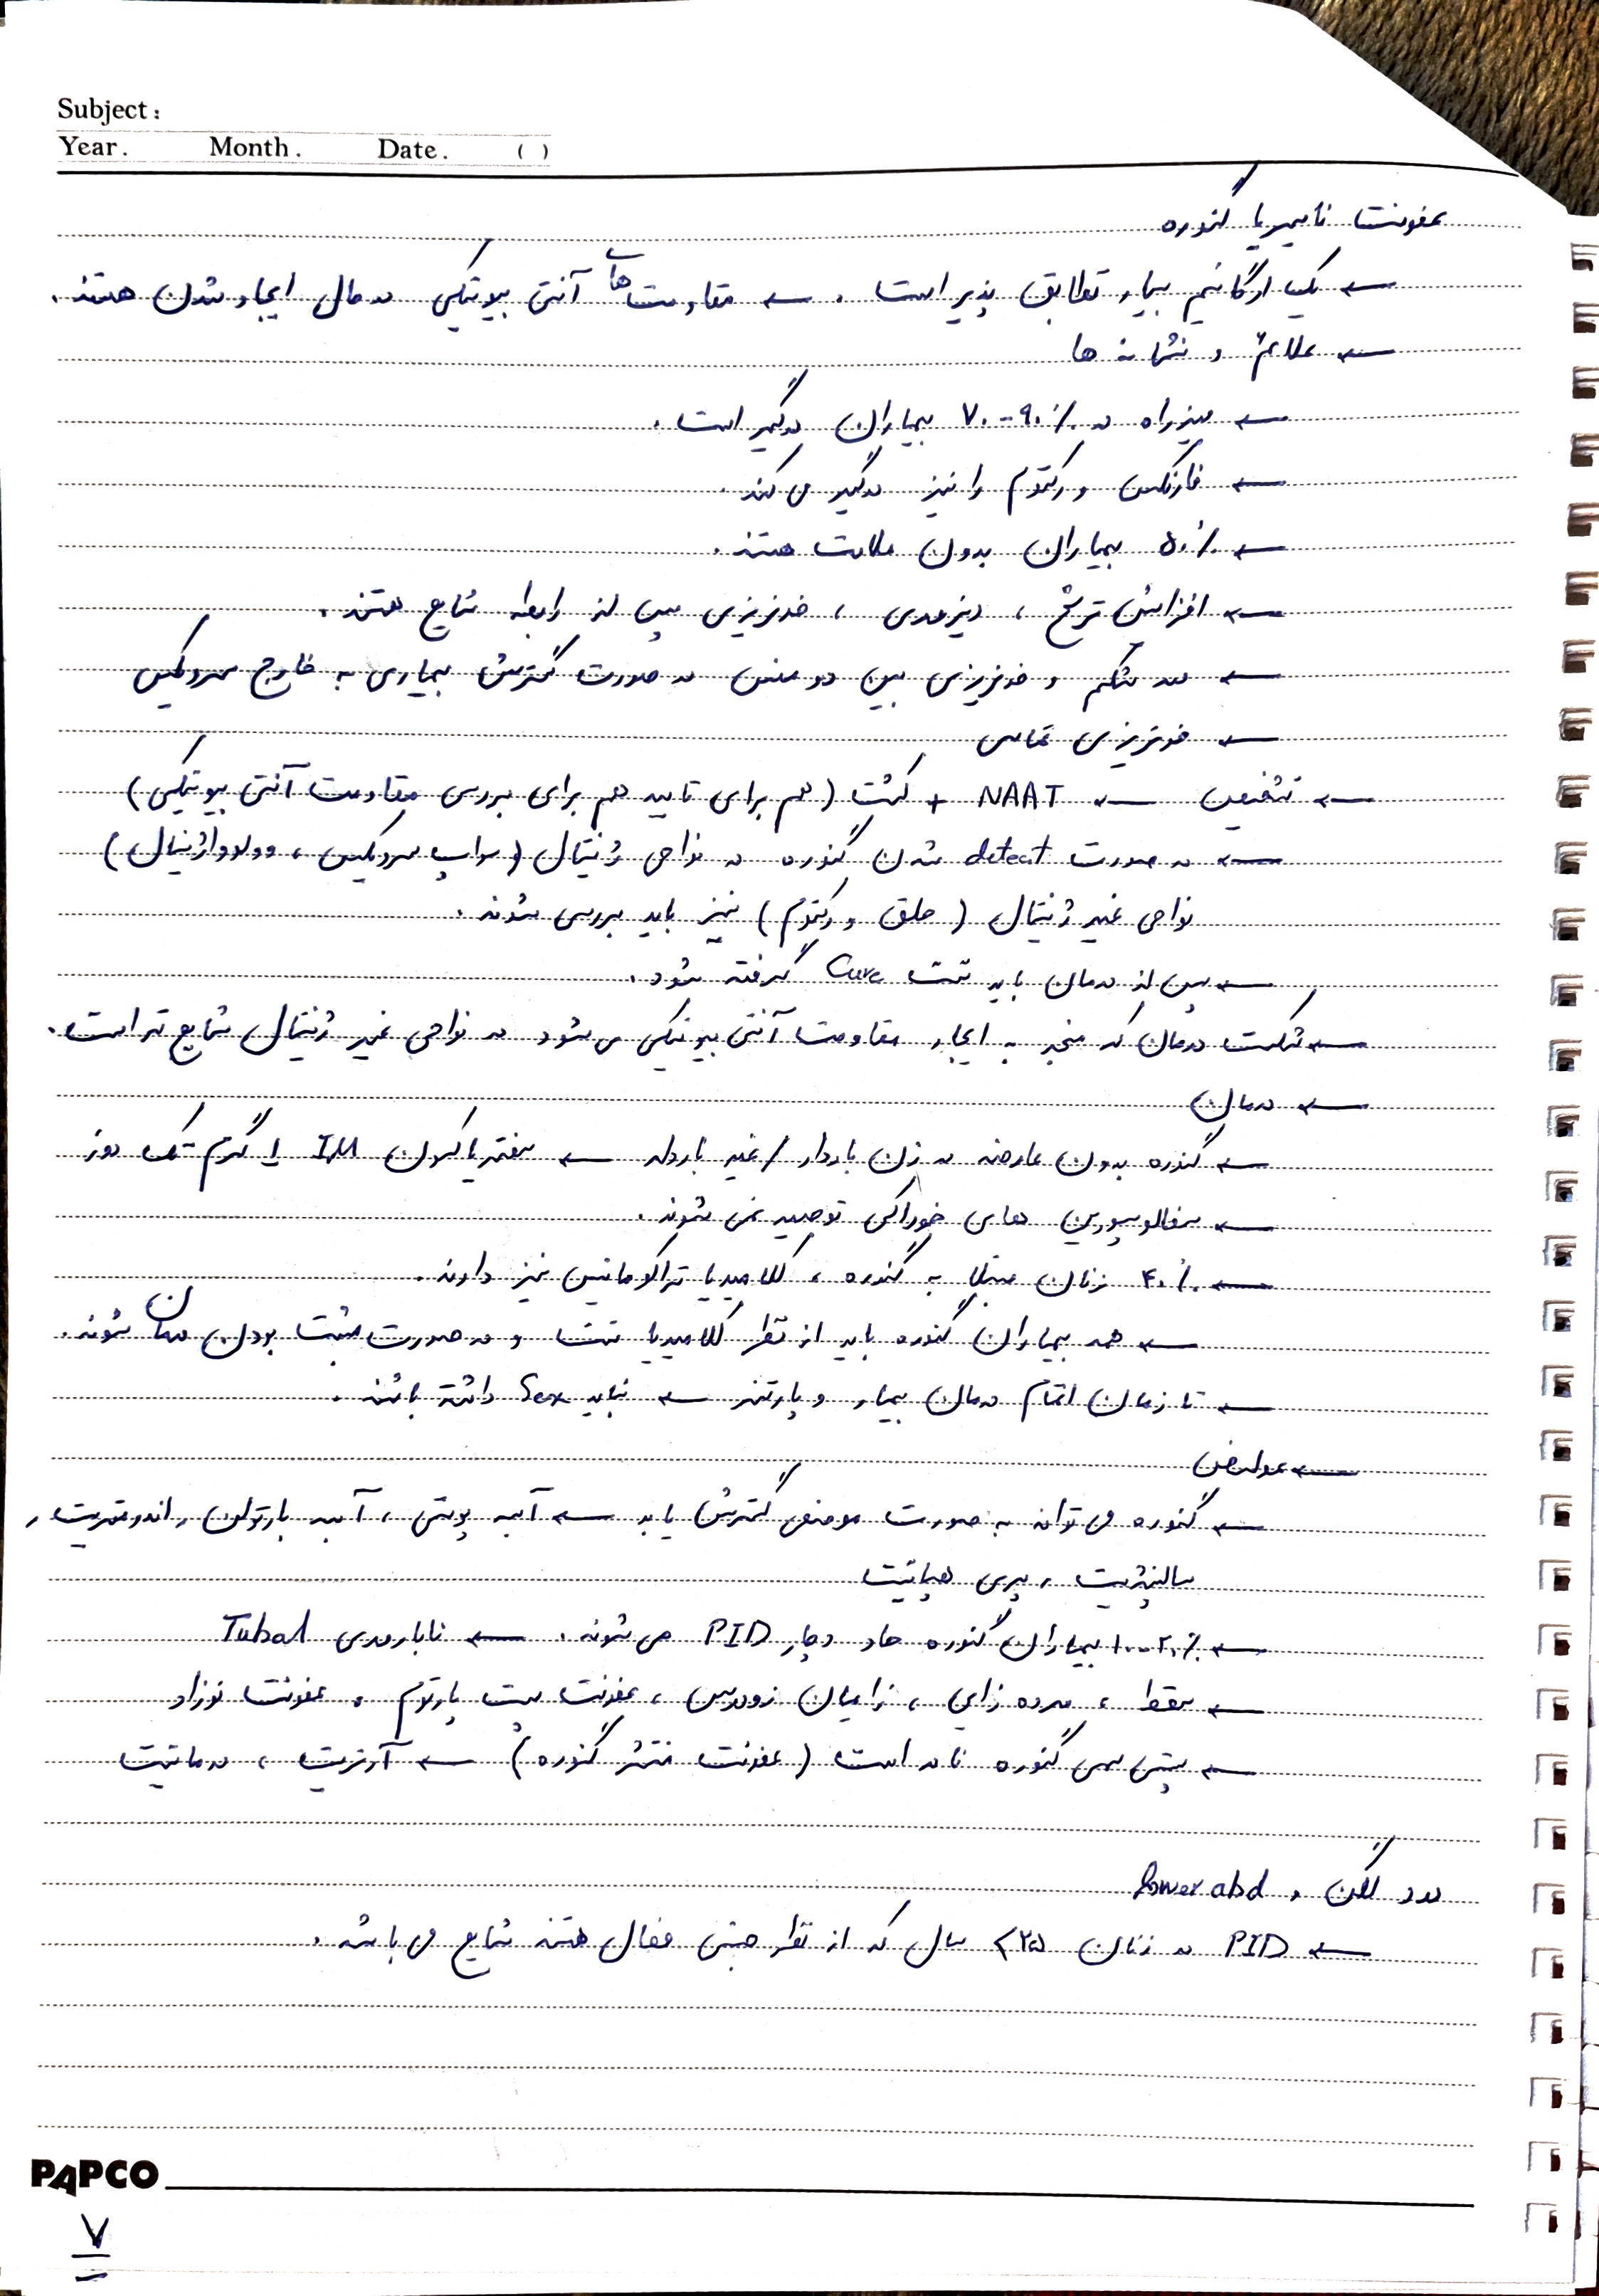
\includegraphics[width=\textwidth,height=0.86\textheight,keepaspectratio]{images/pic07.jpg}
\end{center}
\clearpage
\begin{center}
\textbf{تصویر 8}\par
\lr{\detokenize{20261011_121133751.jpg}}\par
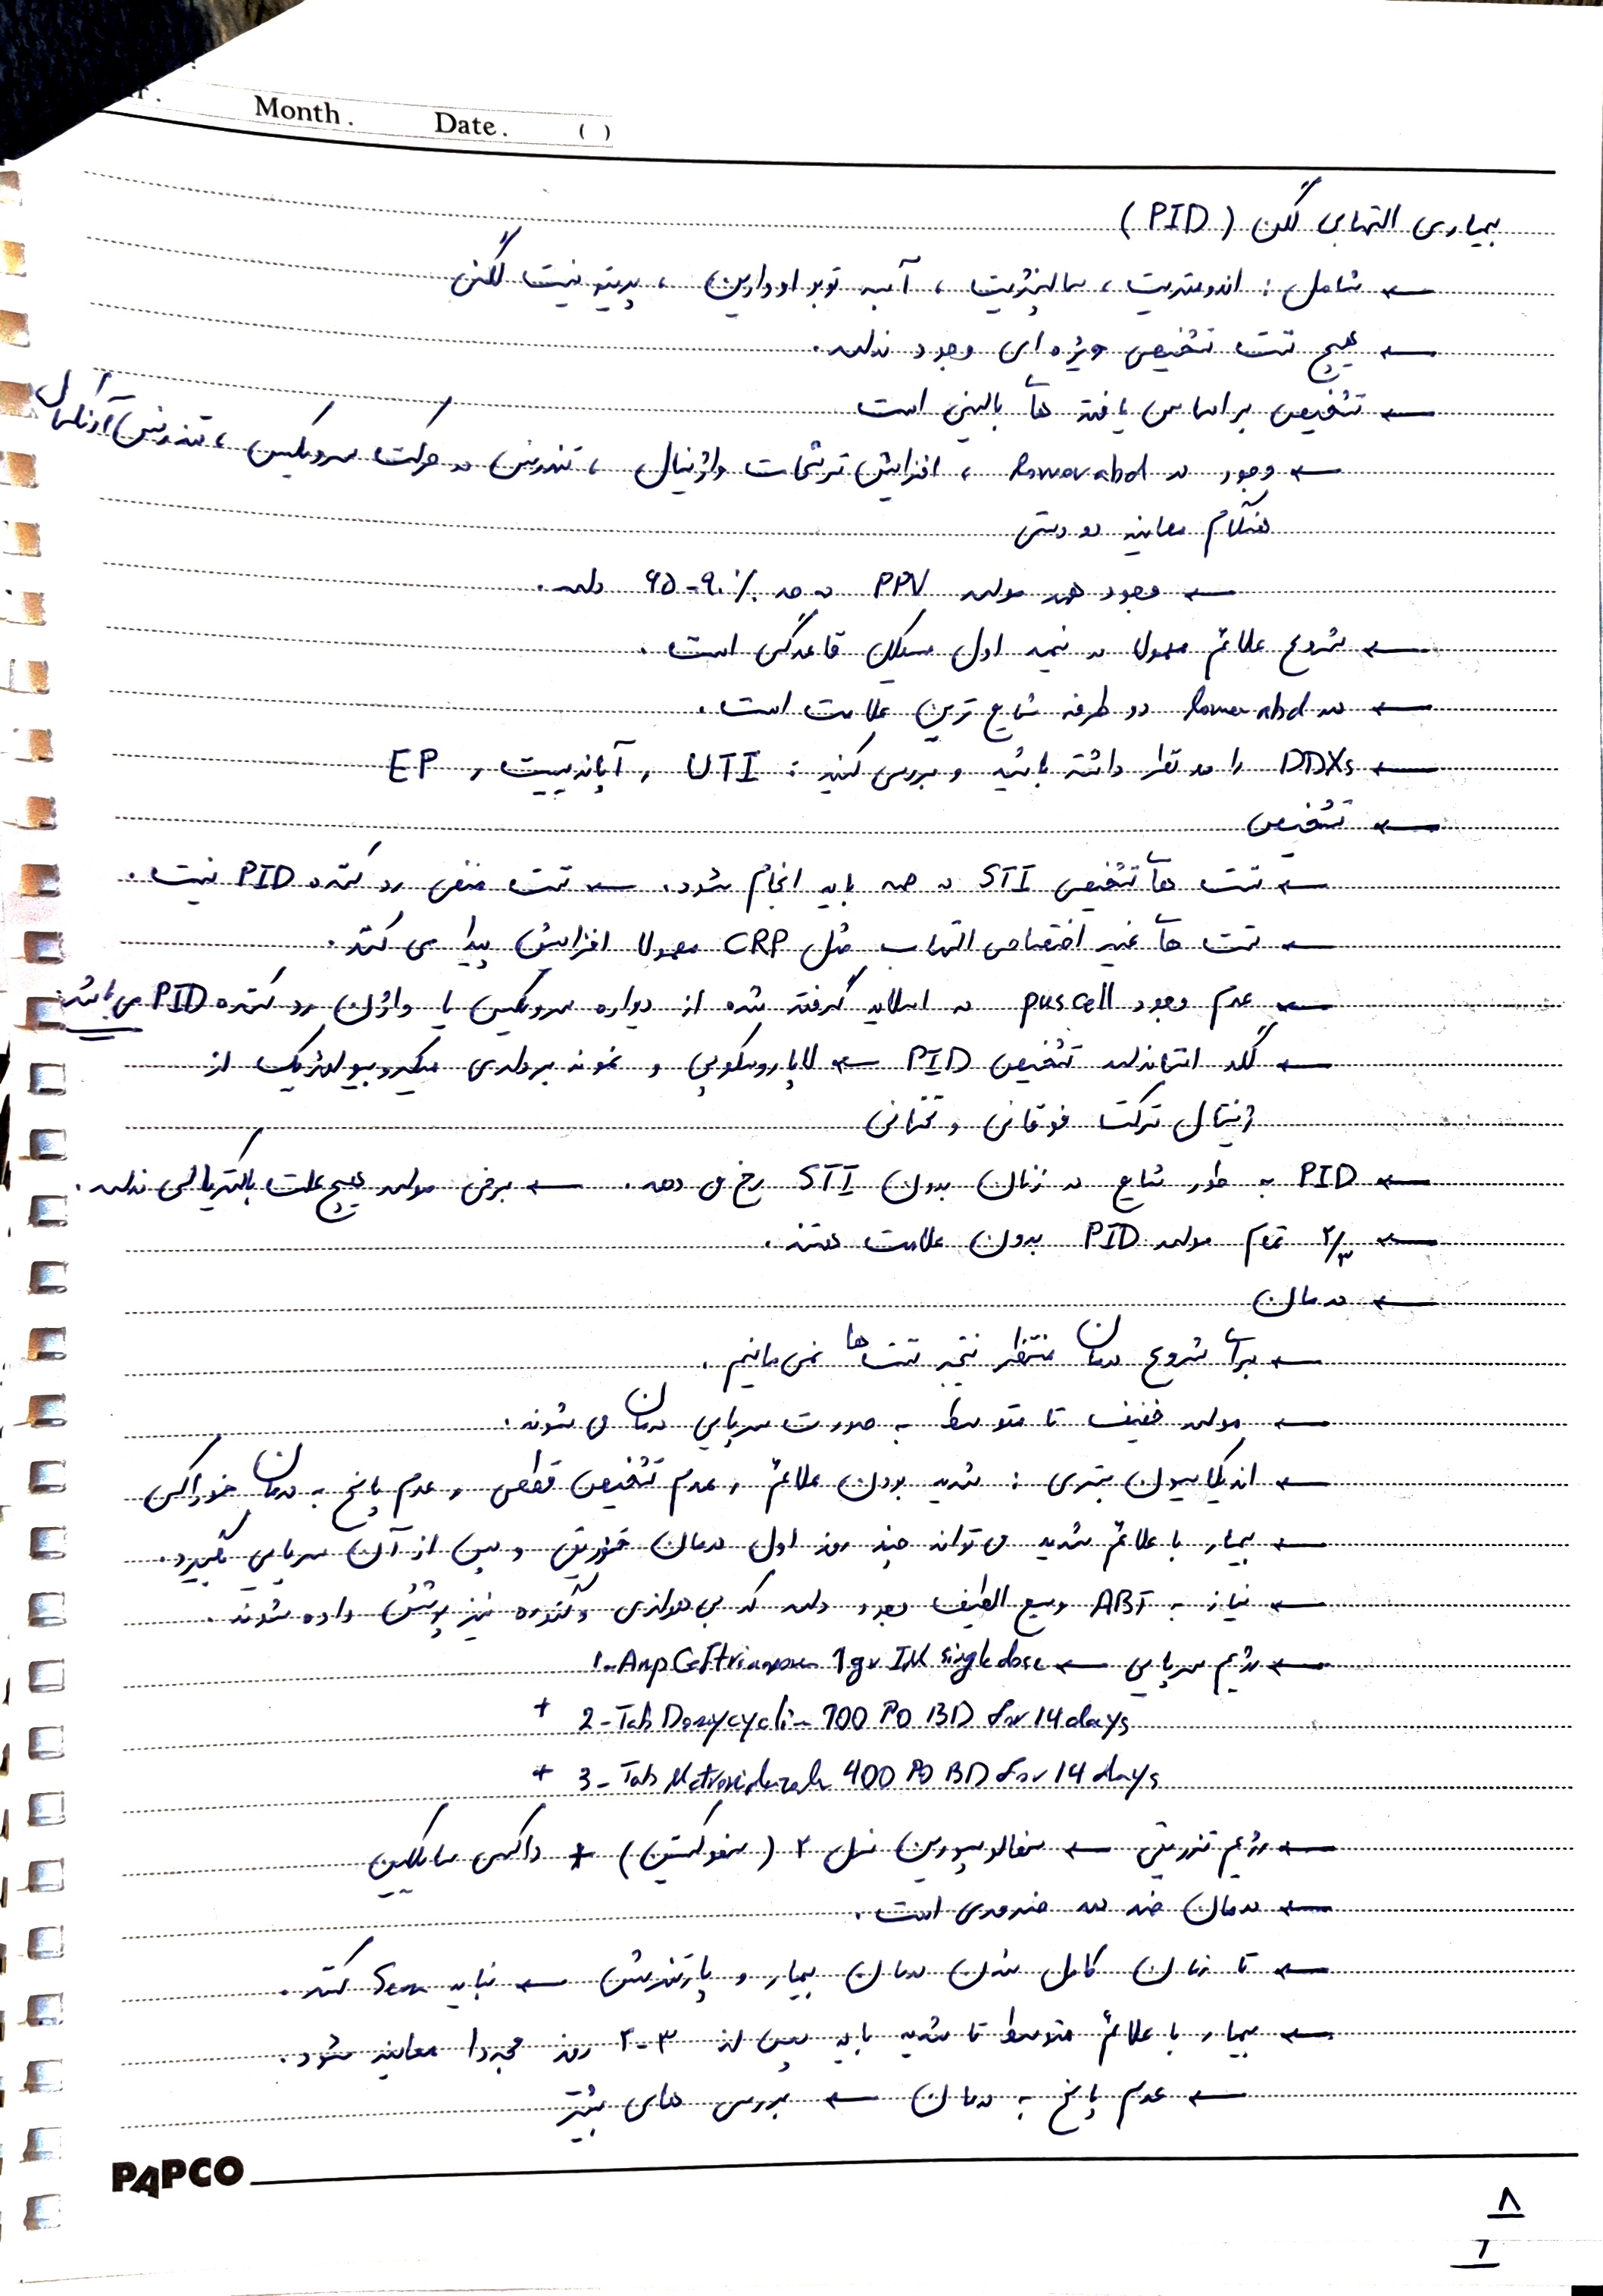
\includegraphics[width=\textwidth,height=0.86\textheight,keepaspectratio]{images/pic08.jpg}
\end{center}
\clearpage
\begin{center}
\textbf{تصویر 9}\par
\lr{\detokenize{20261011_121142023.jpg}}\par
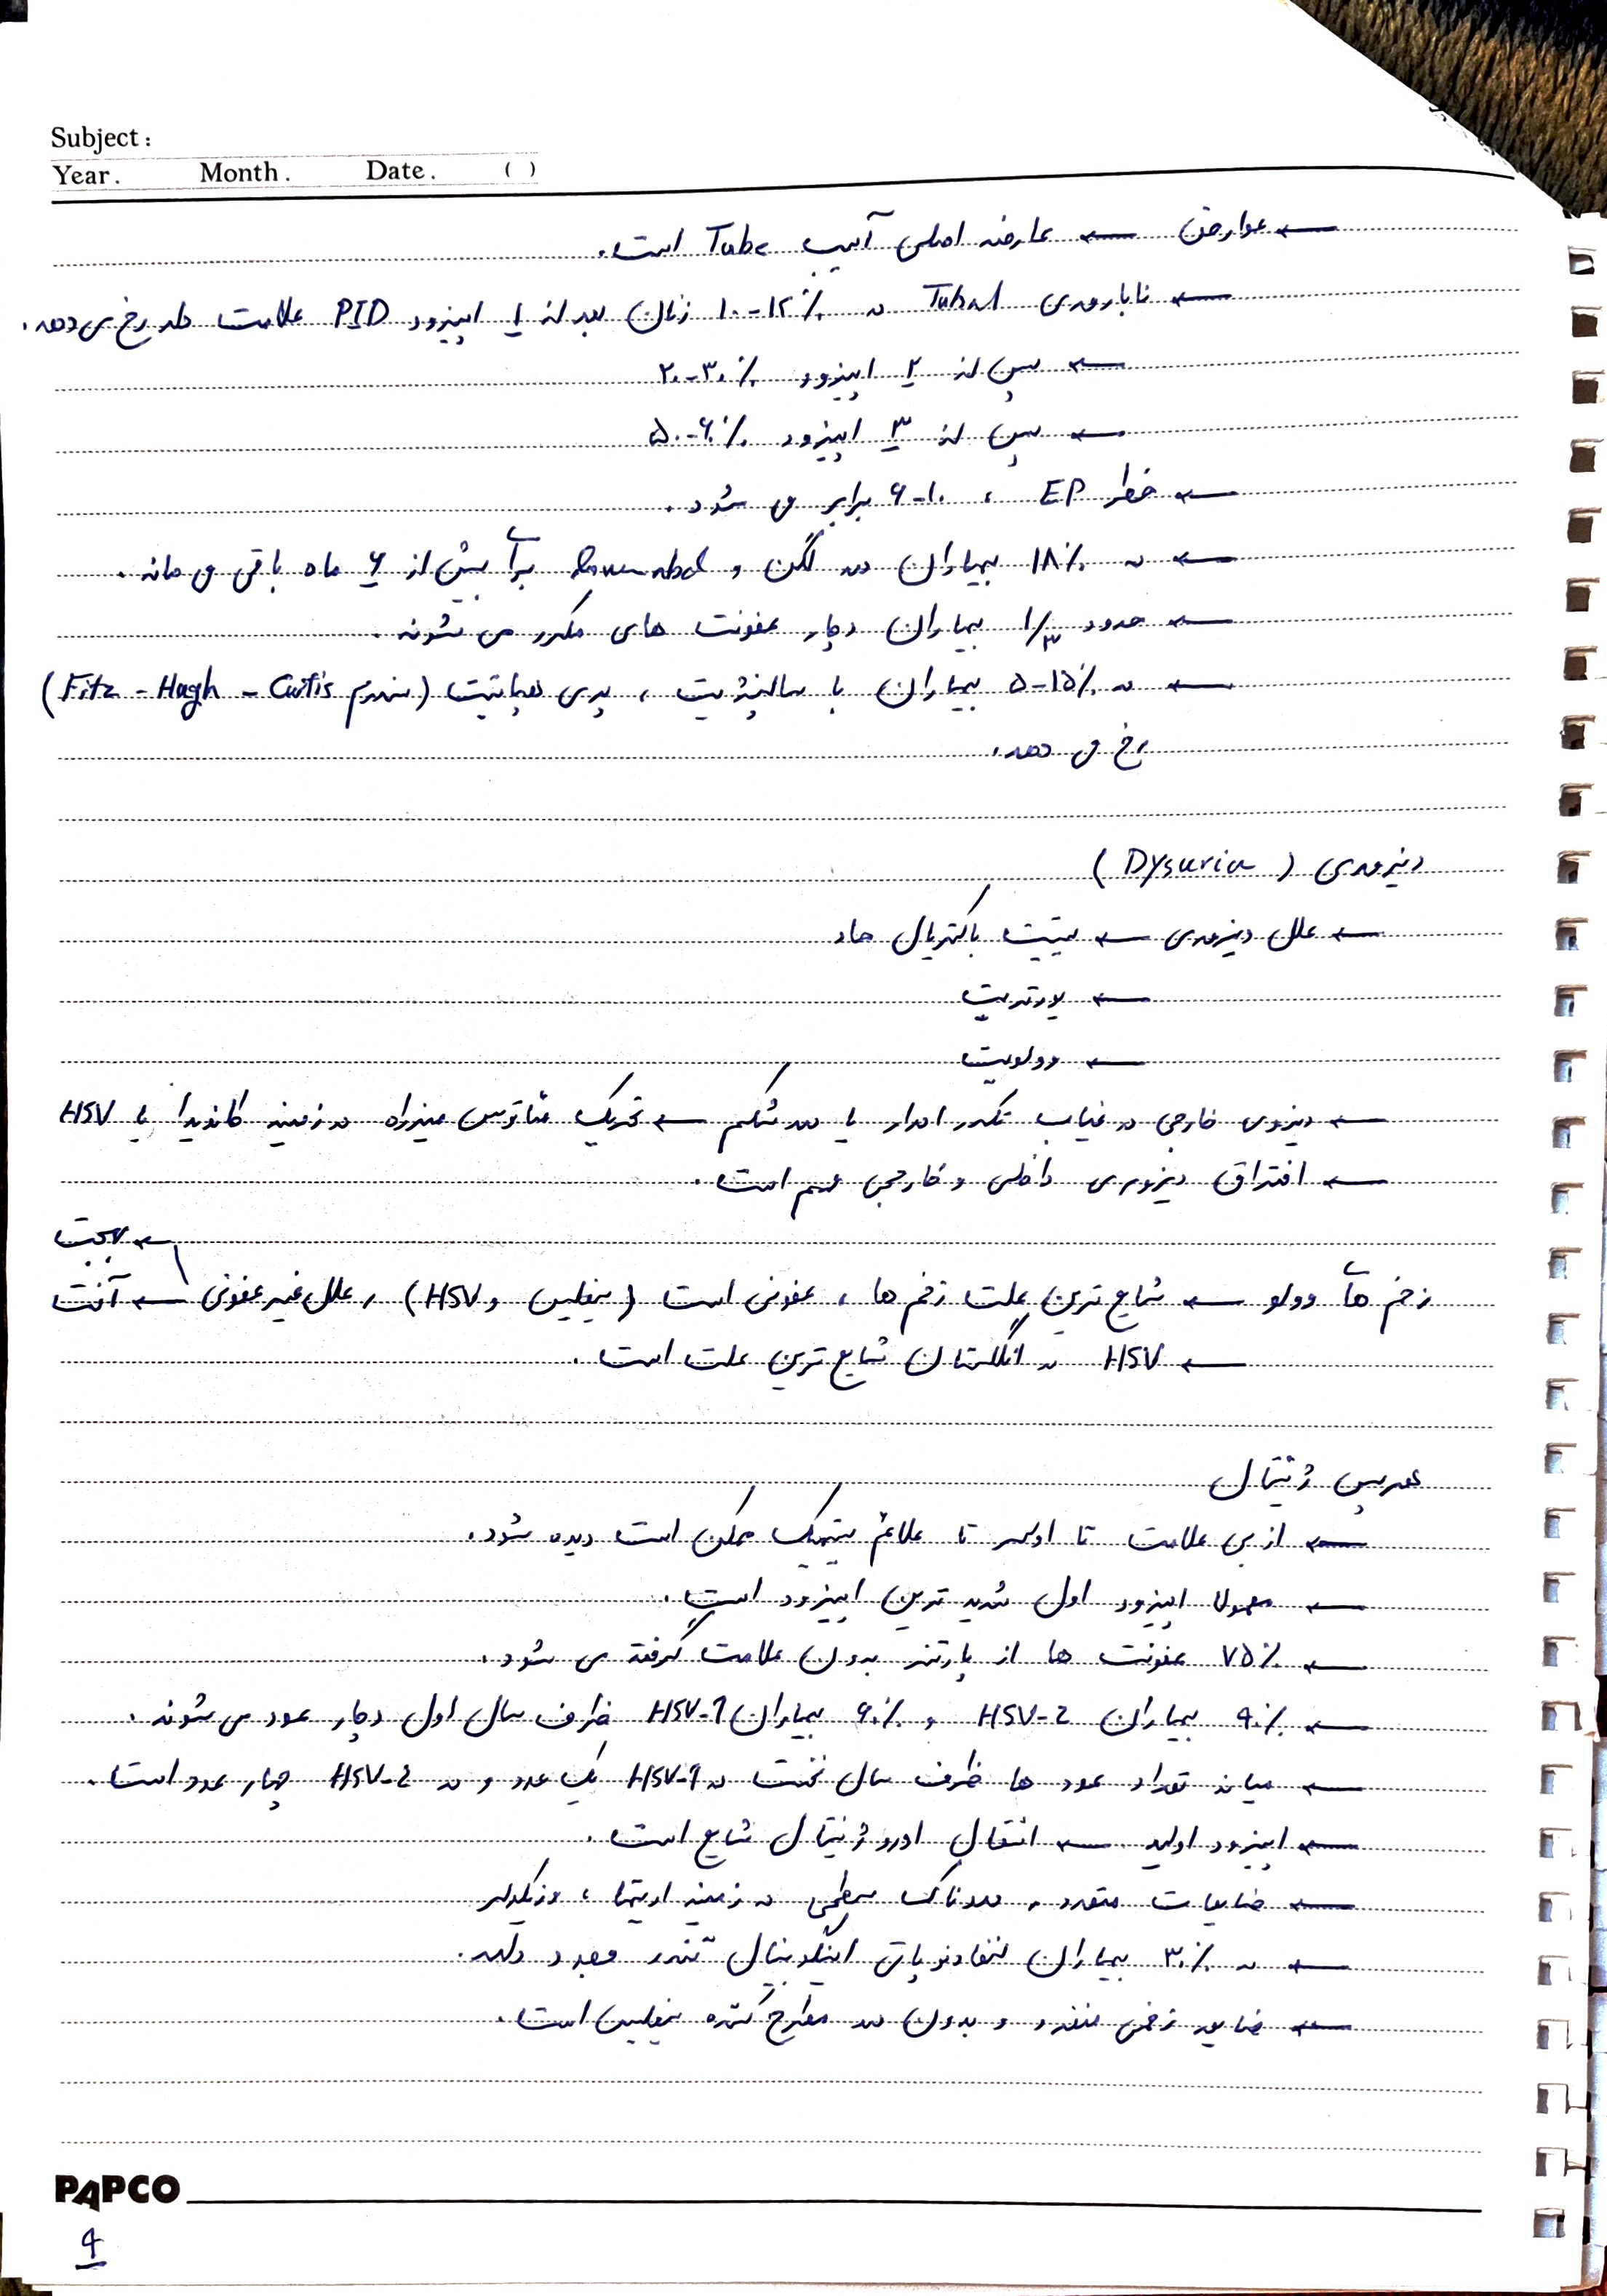
\includegraphics[width=\textwidth,height=0.86\textheight,keepaspectratio]{images/pic09.jpg}
\end{center}
\clearpage
\begin{center}
\textbf{تصویر 10}\par
\lr{\detokenize{20261011_121159146.jpg}}\par
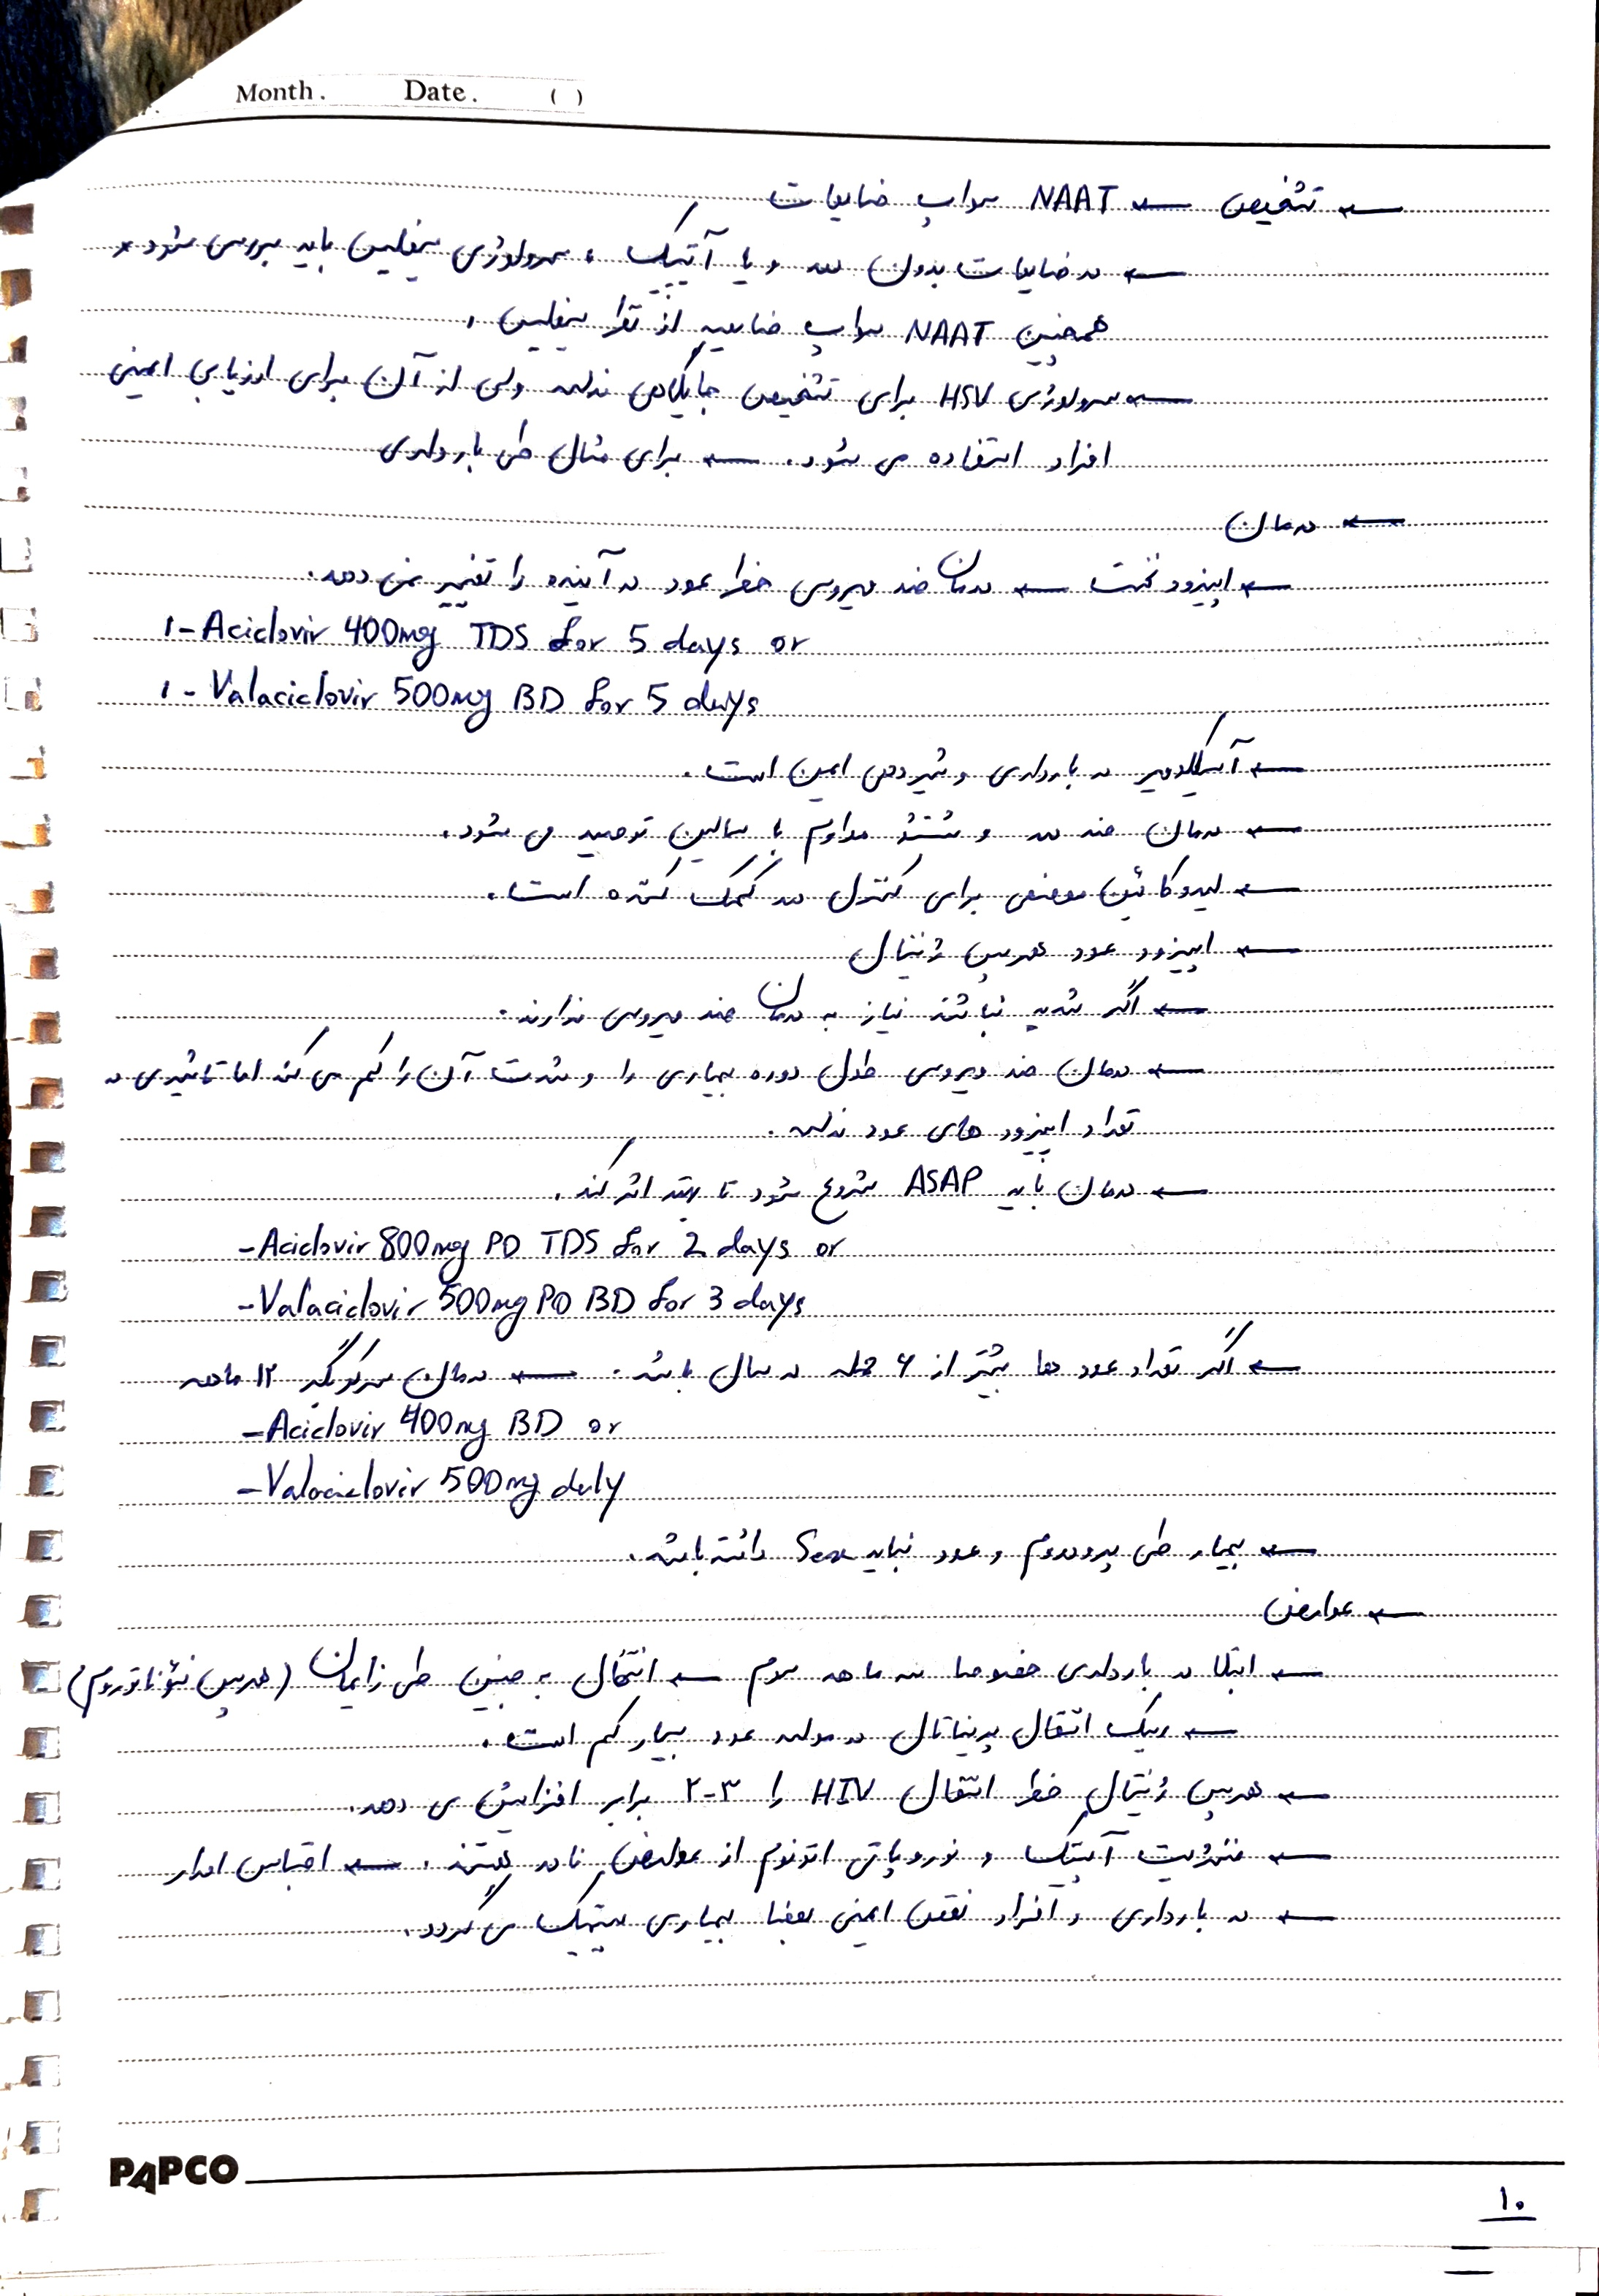
\includegraphics[width=\textwidth,height=0.86\textheight,keepaspectratio]{images/pic10.jpg}
\end{center}
\clearpage
\begin{center}
\textbf{تصویر 11}\par
\lr{\detokenize{20261011_121205075.jpg}}\par
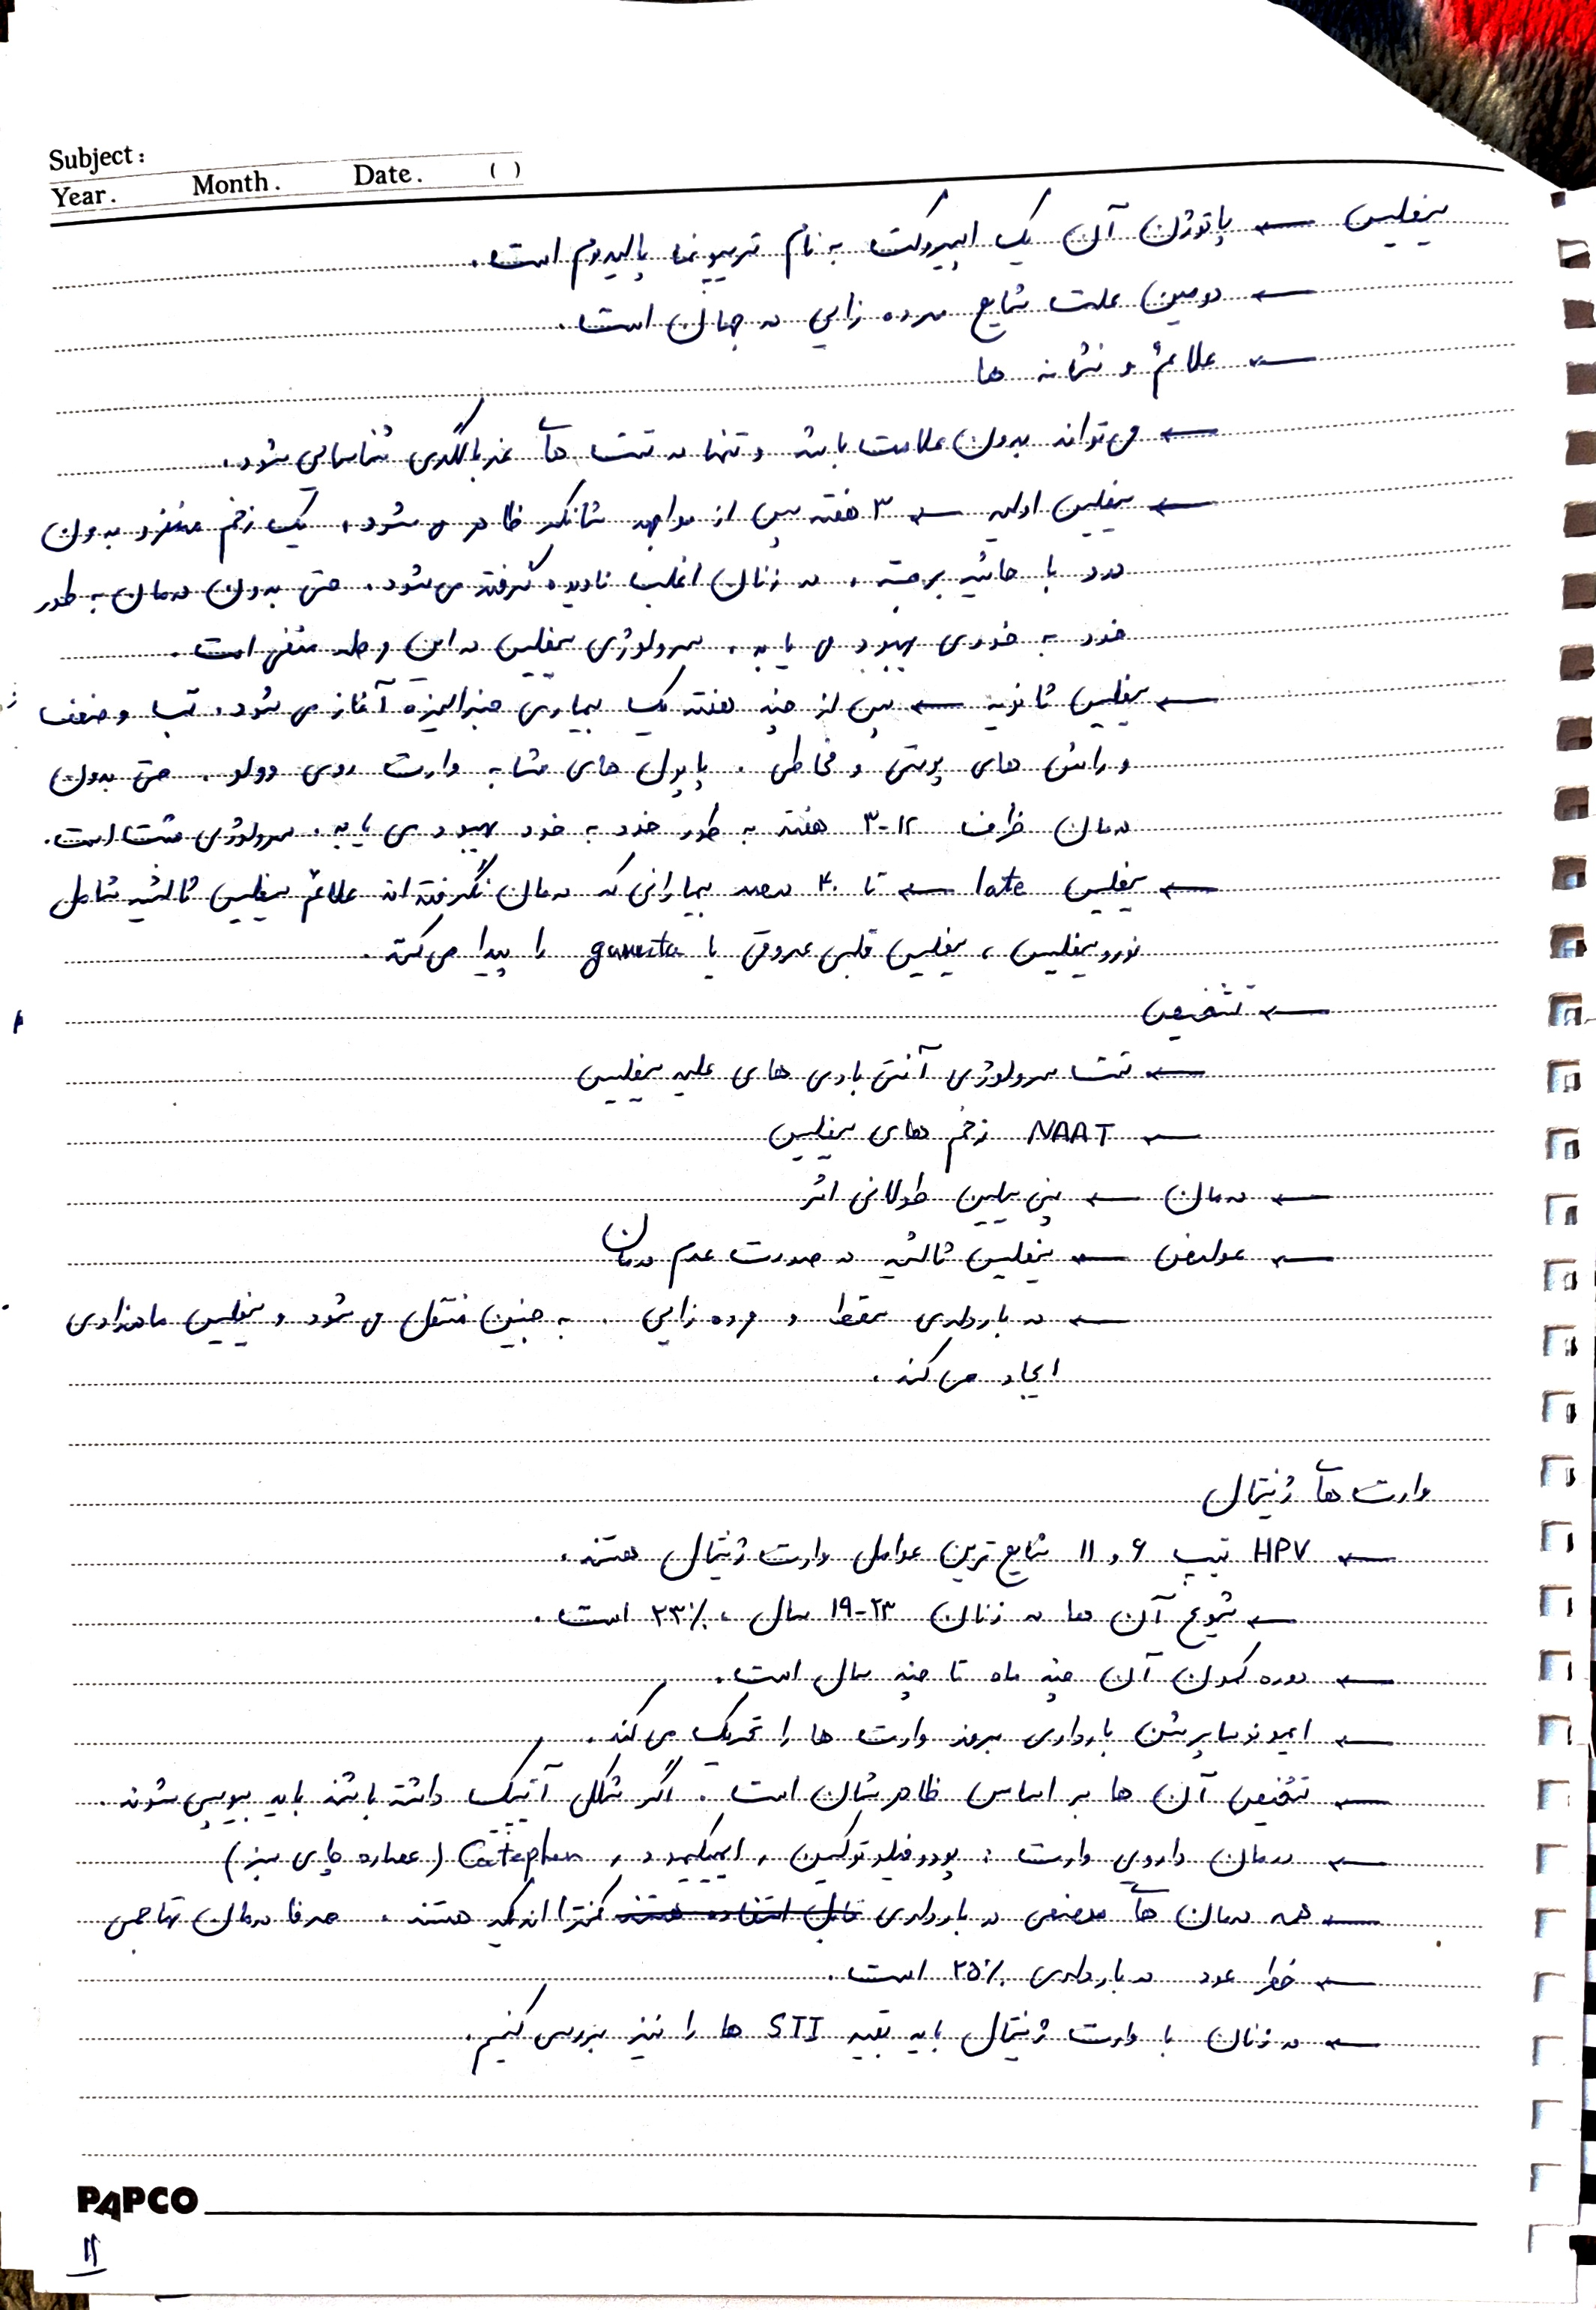
\includegraphics[width=\textwidth,height=0.86\textheight,keepaspectratio]{images/pic11.jpg}
\end{center}
\clearpage
\begin{center}
\textbf{تصویر 12}\par
\lr{\detokenize{20261011_121216949.jpg}}\par
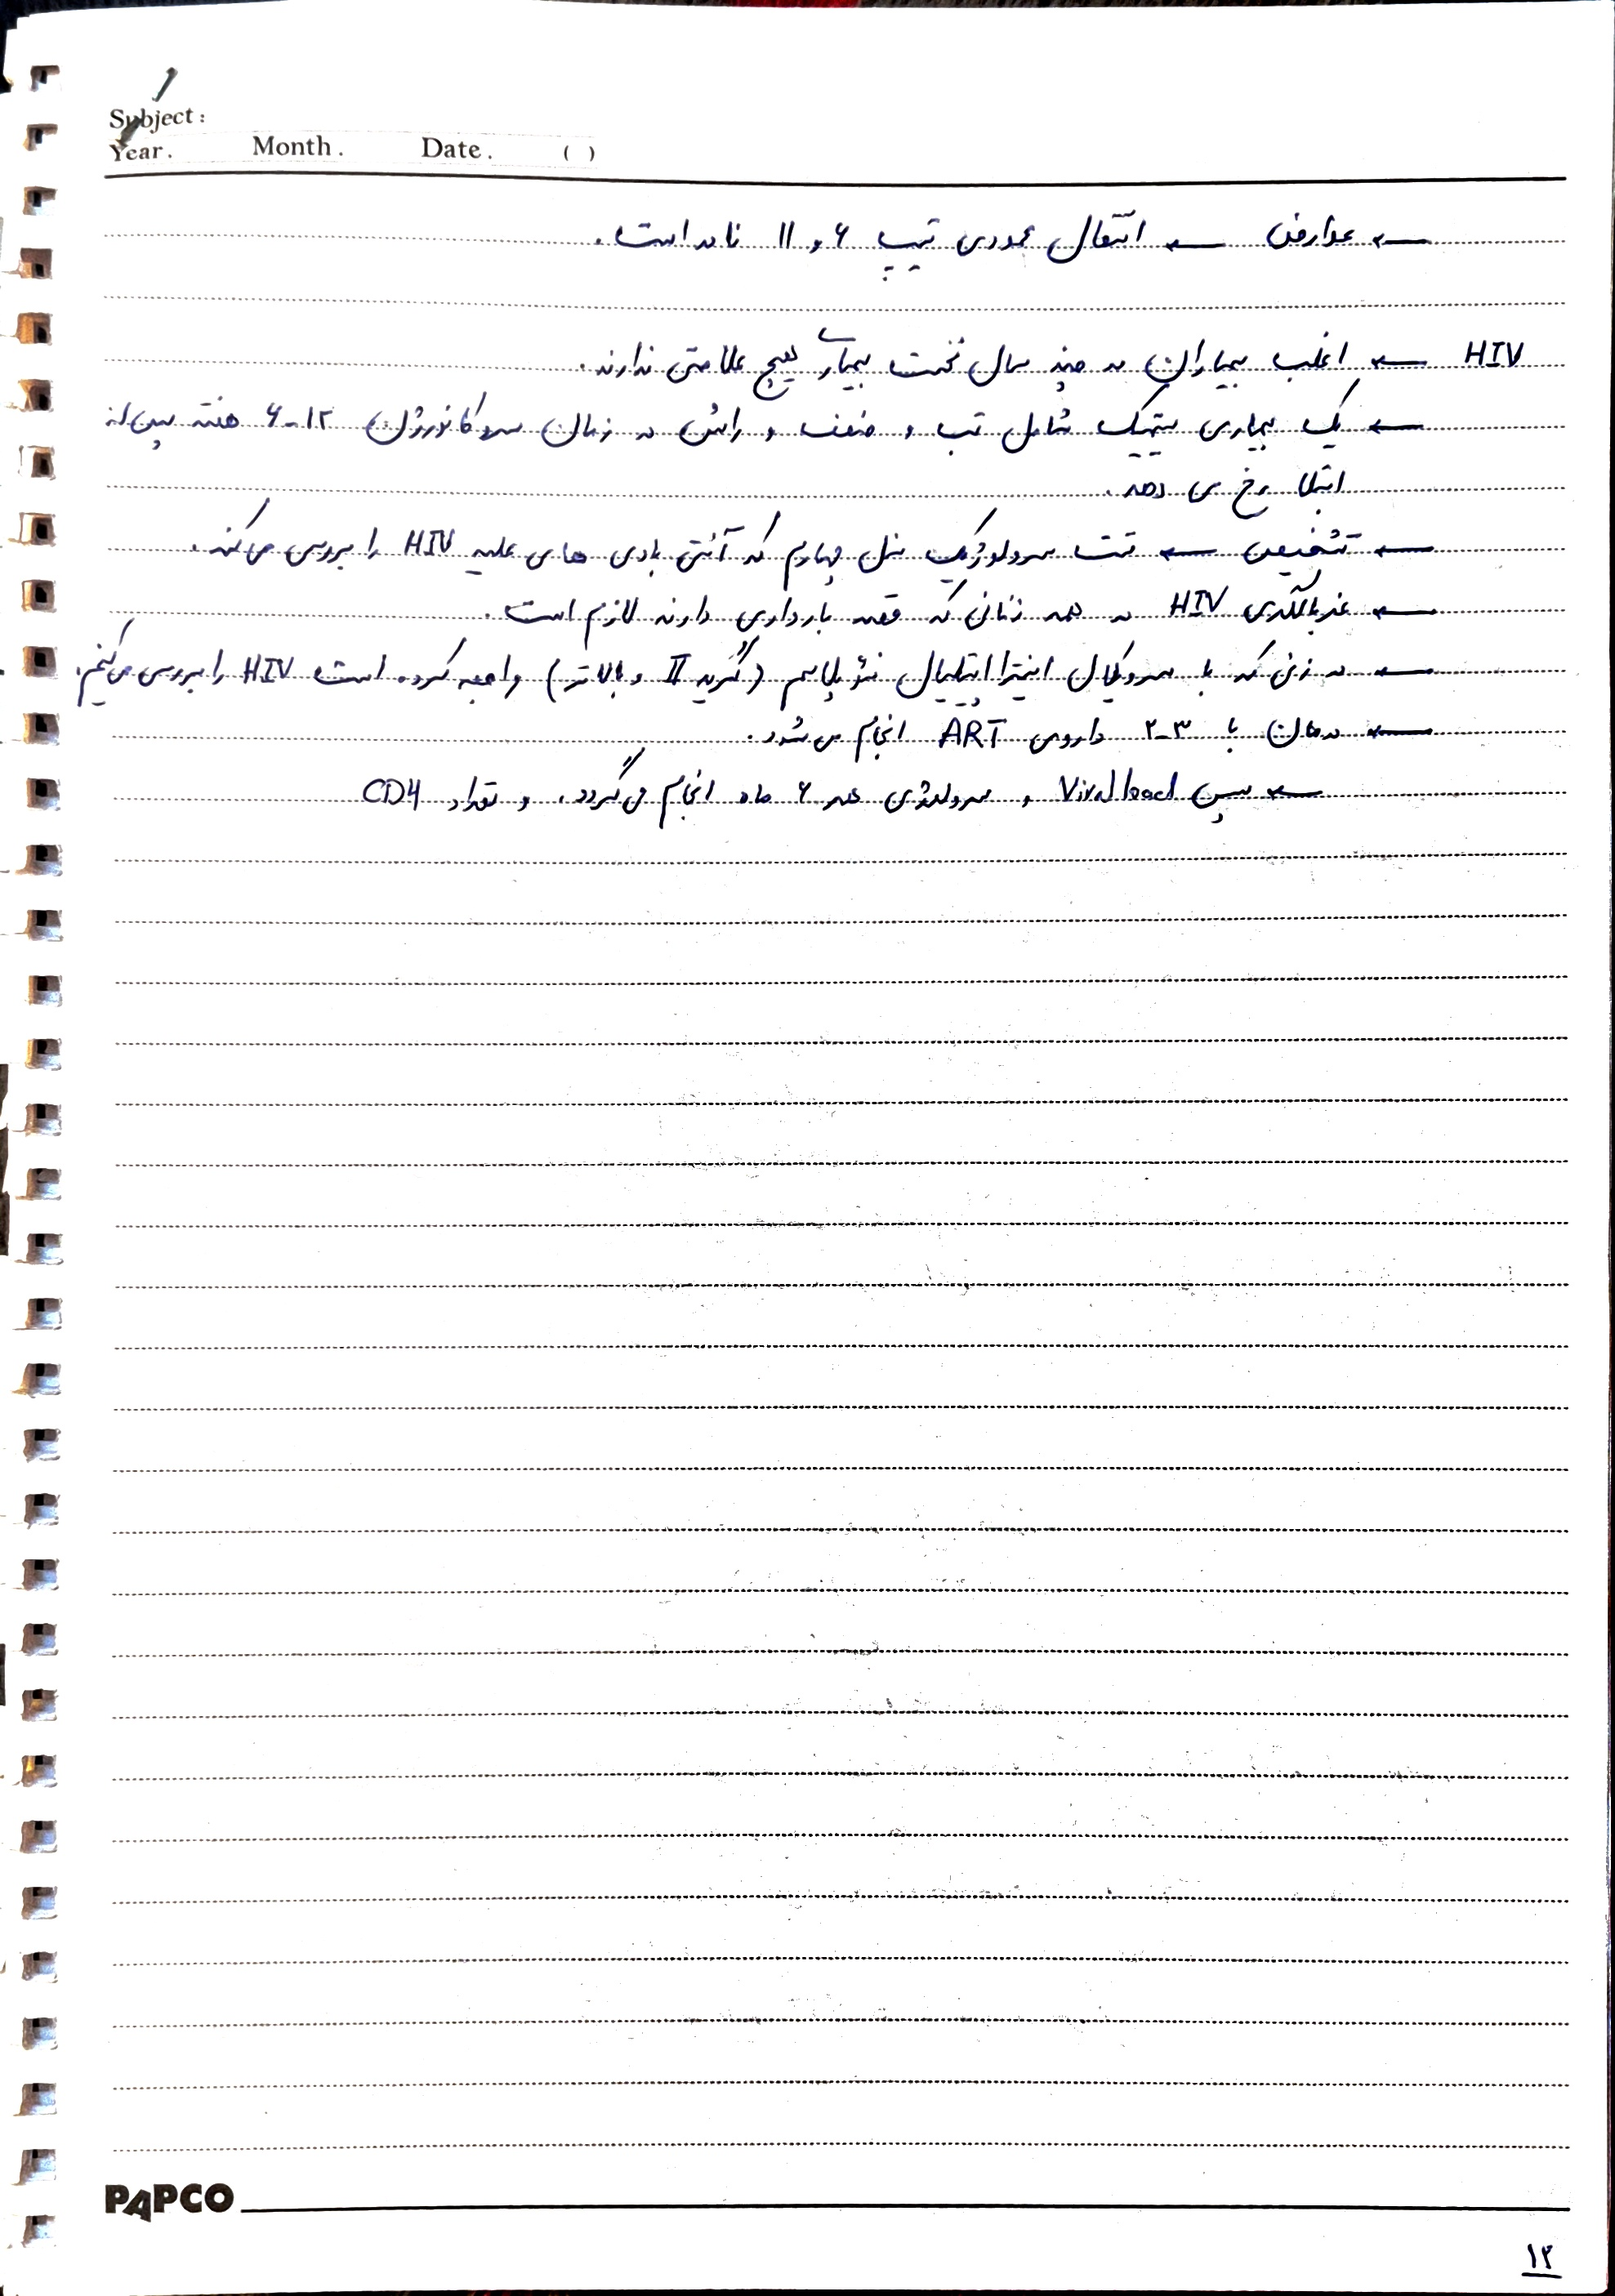
\includegraphics[width=\textwidth,height=0.86\textheight,keepaspectratio]{images/pic12.jpg}
\end{center}
\STIfinish
